% THIS IS AN EXAMPLE DOCUMENT FOR VLDB 2012
% based on ACM SIGPROC-SP.TEX VERSION 2.7
% Modified by  Gerald Weber <gerald@cs.auckland.ac.nz>
% Removed the requirement to include *bbl file in here. (AhmetSacan, Sep2012)
% Fixed the equation on page 3 to prevent line overflow. (AhmetSacan, Sep2012)
%\documentclass{acm_proc_article-sp}
%\documentclass{sig-alternate}
\documentclass{vldb}
%\documentclass{sig-alternate-05-2015}
% The following \documentclass options may be useful:

% preprint      Remove this option only once the paper is in final form.
% 10pt          To set in 10-point type instead of 9-point.
% 11pt          To set in 11-point type instead of 9-point.
% authoryear    To obtain author/year citation style instead of numeric.
%\documentclass{vldb}
\usepackage{graphicx}
\usepackage{balance}  % for  \balance command ON LAST PAGE  (only there!)
\usepackage{xspace}
\usepackage{algorithm}
\usepackage{algpseudocode}
\usepackage{color}
\usepackage{cite}
\usepackage{subfigure}
\usepackage{courier}
\usepackage{enumitem}
\usepackage{url}
\setlist{nosep}
\usepackage{atbegshi}
\usepackage{hyperref}
\usepackage{array}
\usepackage[bottom]{footmisc}
\usepackage[T1]{fontenc}
\usepackage[11pt]{moresize}
\hypersetup{
  colorlinks,
  linkcolor={magenta},
  citecolor={blue},
  urlcolor={magenta}
}
 \usepackage{setspace}
 \usepackage{sidecap}

%For title sections compression (following two lines)
% \usepackage[compact]{titlesec}
% \newcommand{\subparagraph}{}

\makeatletter
\renewcommand{\ALG@beginalgorithmic}{\small}
\makeatother

\let\Algorithm\algorithm
\renewcommand\algorithm[1][]{\Algorithm[#1]\setstretch{1.05}}

\newcommand{\mylabel}[2]{#2\def\@currentlabel{#2}\label{#1}}

\renewcommand{\sectionautorefname}{\S}
\renewcommand{\subsectionautorefname}{\S}
\begin{document}

% ****************** TITLE ****************************************

\newtheorem{definition}{\scriptsize {\small D}EFINITION}
\newtheorem{theorem}{\scriptsize {\small T}HEOREM}
\newtheorem{lemma}{\scriptsize {\small T}HEOREM}
\newcommand{\crossrec}{\textsc{X-Map}\xspace}
\newcommand{\crossrecib}{\textsc{X-Map-ib}\xspace}
\newcommand{\crossrecub}{\textsc{X-Map-ub}\xspace}
\newcommand{\privcrossrec}{\textsc{PX-Map}\xspace}
\newcommand{\npcrossrec}{\textsc{NX-Map}\xspace}
\newcommand{\npcrossrecib}{\textsc{NX-Map-ib}\xspace}
\newcommand{\npcrossrecub}{\textsc{NX-Map-ub}\xspace}
\newcommand{\mixcrossrec}{\texttt{(\hspace{-0.5mm}P\hspace{-0.5mm})\hspace{-1mm}X-Map}\xspace}
\newcommand{\graphsim}{\textsc{X-Sim}\xspace}
\newcommand{\framework}{\textsc{X-Ware}\xspace}
\renewcommand{\algorithmicrequire}{\textbf{Input:}}
\renewcommand{\algorithmicensure}{\textbf{Output:}}
\newcommand\Algphase[1]{%
\vspace*{-.7\baselineskip}\Statex\hspace*{\dimexpr-\algorithmicindent-2pt\relax}\rule{0.48\textwidth}{0.4pt}%
\Statex\hspace*{-\algorithmicindent}\textbf{#1}%
\vspace*{-.7\baselineskip}\Statex\hspace*{\dimexpr-\algorithmicindent-2pt\relax}\rule{0.48\textwidth}{0.4pt}%
}

\setlength{\abovedisplayskip}{-0.8pt}
\setlength{\belowdisplayskip}{-0.8pt}
\setlength{\textfloatsep}{0pt}



\title{What You Might Like To Read After Watching Interstellar}

% possible, but not really needed or used for PVLDB:
%\subtitle{[Extended Abstract]
%\titlenote{A full version of this paper is available as\textit{Author's Guide to Preparing ACM SIG Proceedings Using \LaTeX$2_\epsilon$\ and BibTeX} at \texttt{www.acm.org/eaddress.htm}}}

% ****************** AUTHORS **************************************

% You need the command \numberofauthors to handle the 'placement
% and alignment' of the authors beneath the title.
%
% For aesthetic reasons, we recommend 'three authors at a time'
% i.e. three 'name/affiliation blocks' be placed beneath the title.
%
% NOTE: You are NOT restricted in how many 'rows' of
% "name/affiliations" may appear. We just ask that you restrict
% the number of 'columns' to three.
%
% Because of the available 'opening page real-estate'
% we ask you to refrain from putting more than six authors
% (two rows with three columns) beneath the article title.
% More than six makes the first-page appear very cluttered indeed.
%
% Use the \alignauthor commands to handle the names
% and affiliations for an 'aesthetic maximum' of six authors.
% Add names, affiliations, addresses for
% the seventh etc. author(s) as the argument for the
% \additionalauthors command.
% These 'additional authors' will be output/set for you
% without further effort on your part as the last section in
% the body of your article BEFORE References or any Appendices.

%\numberofauthors{8} %  in this sample file, there are a *total*
% of EIGHT authors. SIX appear on the 'first-page' (for formatting
% reasons) and the remaining two appear in the \additionalauthors section.

\numberofauthors{3} %  in this sample file, there are a *total*
% of EIGHT authors. SIX appear on the 'first-page' (for formatting
% reasons) and the remaining two appear in the \additionalauthors section.

\author{
% You can go ahead and credit any number of authors here,
% e.g. one 'row of three' or two rows (consisting of one row of three
% and a second row of one, two or three).
%
% The command \alignauthor (no curly braces needed) should
% precede each author name, affiliation/snail-mail address and
% e-mail address. Additionally, tag each line of
% affiliation/address with \affaddr, and tag the
% e-mail address with \email.
%
% 1st. author
\alignauthor
\hspace{-4mm}
Rachid Guerraoui\\
\hspace{-4mm}
       \affaddr{EPFL}\\
       \email{\hspace{-4mm}rachid.guerraoui@epfl.ch}
% 2nd. author
\alignauthor
\hspace{-14mm}
Anne-Marie Kermarrec\\
\hspace{-14mm}
       \affaddr{Inria}\\
       \email{\hspace{-14mm}anne-marie.kermarrec\\\hspace{-14mm}@inria.fr}
% 3rd. author
\alignauthor 
\hspace{-35mm}
Tao Lin\\
\hspace{-35mm}
       \affaddr{EPFL}\\
       \email{\hspace{-35mm}tao.lin@epfl.ch}
%\and  % use '\and' if you need 'another row' of author names
% 4th. author
\alignauthor
\hspace{-60mm}
Rhicheek Patra\\
\hspace{-60mm}
       \affaddr{EPFL}\\
       \email{\hspace{-60mm}rhicheek.patra@epfl.ch}
       %\email{\hspace{-60mm}jean-ronan.vigouroux\\\hspace{-60mm}@technicolor.com}
}

%\titlenote{Authors appear in alphabetical order.}

% There's nothing stopping you putting the seventh, eighth, etc.
% author on the opening page (as the 'third row') but we ask,
% for aesthetic reasons that you place these 'additional authors'
% in the \additional authors block, viz.
% Just remember to make sure that the TOTAL number of authors
% is the number that will appear on the first page PLUS the
% number that will appear in the \additionalauthors section.


\maketitle



\begin{abstract}
Recommenders are widely implemented nowadays by major e-commerce players like Netflix, Amazon or Last.fm. They typically make use of effective collaborative filtering schemes to select the most relevant items to suggest. However, most recommenders today are \emph{homogeneous}: they focus on a specific domain (e.g., either movies or books). In short, Alice will only get recommended a movie if she has been rating only movies. Clearly, the multiplicity of web applications is calling for \emph{heterogeneous} recommendations. Ideally, Alice should be able to get recommendations for books even if she has only rated movies.
%Basically, Alice should be recommended books based on her past rating of movies and Bob should be recommended movies based on his past rating of books. 
% Yet, heterogeneity opens new challenges for computing \emph{similarity}, protecting \emph{privacy} and ensuring \emph{scalability}.

In this paper, we present \crossrec, a heterogeneous recommender addressing such issues. \crossrec relies on \graphsim, a novel meta path-based similarity where a \emph{meta path} is a path consisting of heterogeneous items (like movies, books). \graphsim computes the transitive closure of inter-item similarities over several domains based on users who rated across these domains. \graphsim is then used to generate a user profile (called \emph{AlterEgo}) for a domain where the user might not have any activity yet. Furthermore, information aggregation across multiple domains also increases the potential privacy risk for users. \crossrec employs differential privacy to address such privacy concerns.

%We show how to do that, while ensuring differential privacy, and then generate relevant recommendations in that domain.
% \crossrec applies an exponential technique to determine the probability of item selection and ensure differential privacy. scalability is ensured using a layer-based selection technique. 

We present a comprehensive experimental evaluation of \crossrec using real traces from Amazon. Our evaluation shows that, in terms of recommendation quality, \crossrec outperforms alternative heterogeneous recommenders, and in terms of throughput, \crossrec scales linearly with increasing number of machines.


%Our evaluation shows that \crossrec, without any privacy overhead, significantly outperforms alternative heterogeneous recommenders whereas it still provides slightly better quality than the alternatives with the additional privacy overhead. We also show that \crossrec delivers near-linear scalability with an increasing number of machines.


\end{abstract}



% A category with the (minimum) three required fields
%\category{H.4}{Information Systems Applications}{Miscellaneous}
%A category including the fourth, optional field follows...
%\category{D.2.8}{Software Engineering}{Metrics}[complexity measures, performance measures]

%\terms{Theory}

%\keywords{ACM proceedings, \LaTeX, text tagging} % NOT required for Proceedings

\section{Introduction}
\label{intro}
The vast amount of information available in the Internet calls for \emph{personalization} schemes~\cite{bonett2001personalization}, such as \emph{recommenders}, that aid the users in their web navigation activities. Recommenders seek to suggest \emph{relevant} items to users based on their interests, by typically relying on \emph{Collaborative Filtering} (CF) algorithms~\cite{resnick1994grouplens} to leverage similarities between users. Such similarities are computed using the past rating histories of users. The axiom here is that  \emph{if Alice and Bob have liked the same items in the past, they are likely to be interested in the same items in the future}. 


\begin{figure}
\begin{center}
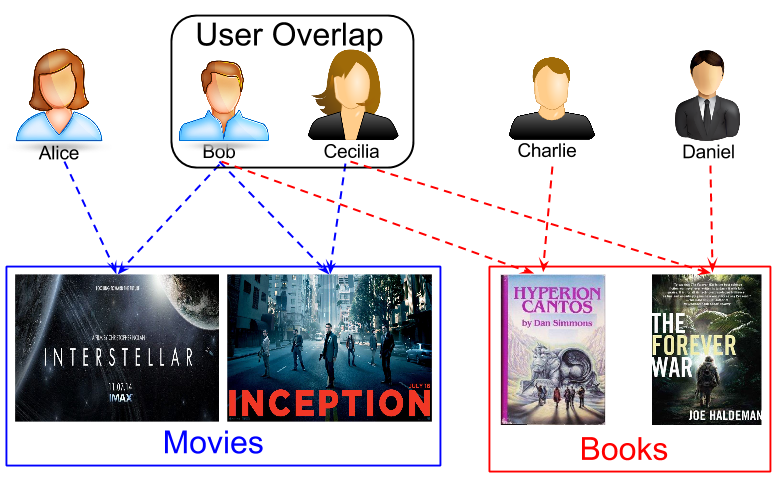
\includegraphics[height=1.7in,width=2.8in]{figures/Overlap.png}
\vspace{-4mm}
\caption{{\bf User overlap (Bob, Cecilia) with heterogeneous personalization.}}
\label{fig:overlap}
\end{center}
\end{figure}

\subsection{Motivation}


However, although widely used today, recommenders are mainly applied in a \emph{homogeneous} sense. Movie recommenders like IMDb or Netflix, news recommenders  like Google News or Yahoo News, as well as music recommenders  like Last.fm and Spotify, each focuses on a specific domain. In short, you will be recommended books if you rated books, and you will be recommended movies if you rated movies. Given the growing multiplicity of web applications, as well as  the amount of information available in the Internet, homogeneity is a major limitation. In short, with most state-of-the-art recommenders, Alice who just joined a book-oriented web application, and never rated any book before, cannot be recommended any relevant book, even if she has been rating many movies and news.

We argue that the next level to personalization is \emph{heterogeneity}, namely \emph{personalization across multiple domains}~\cite{cremonesi2011cross}. Heterogeneous preferences on the web, i.e., preferences from multiple domains, can be leveraged to improve personalization, not only for users who are new to a given domain (\emph{cold-start} situation), but also when the data is \emph{sparse}~\cite{adomavicius2005toward} (e.g, very few ratings per user). In a heterogeneous personalization scheme, if a user, say Alice, liked \emph{Interstellar}, then the system could recommend her books such as \emph{The Forever War} by Joe Haldeman. The intuition is expressed in the scenario depicted in Figure \ref{fig:overlap} where five users rated \emph{at most} one book. First, we make the following observations.
\begin{enumerate}[label=\textnormal{(\arabic*)}]
\item Alice and Bob are like-minded as both like \emph{Interstellar}\label{itm:1}.
\item Bob and Cecilia are like-minded as both like \emph{Inception}\label{itm:2}.
\item Alice and Cecilia have no common interests\label{itm:3}.
\item Alice and Cecilia are only related through Bob\label{itm:4}.
\end{enumerate}

Based on the observations \ref{itm:1}, \ref{itm:2} and \ref{itm:4}, \emph{The Forever War} could be recommended to Alice. Note that if we consider both domains as a single aggregated domain, this heterogeneous recommendation would be less likely due to the observation \ref{itm:3}.

 Heterogeneous personalization improves the quality of recommendation but it also raises several privacy concerns. For example, the new connection between Alice and Cecilia provides the opportunity for a curious user, say Alice, to discover the people (like Bob or Cecilia) who form a bridge between these two domains. She can actually probe to determine the item(s) that allows her to get this recommendation. The probing is done by masquerading as another user and incrementally rating items until the recommendation is made. By itself, her knowledge of such information poses no risk, but when used in conjunction with other information it fills a gap in knowledge that could be key to identifying the other user(s). This is similar to the privacy risk inherent in allowing statistical database queries where it is possible to make inferences from combinations of queries. Such privacy risks are amplified when the domains are owned by different companies (like IMDb for movies and Goodreads for books) which could lead to serious privacy violations.

%{\color{red} ADD MOTIVATION ABOUT PRIVACY COMPANY-BASED VS ACROSS COMPANIES}


\subsection{Challenges}

Building a simple heterogeneous recommender is straightforward by integrating ratings from both domains as a single domain. 
%Some existing work aims to address this heterogeneity problem by integrating ratings from both domains as a single domain~\cite{berkovsky2007distributed,winoto2008if, berkovsky2007cross}.
Following the aforementioned intuition (observation \ref{itm:3}), existing homogeneous personalization schemes~\cite{schafer2007collaborative, resnick1994grouplens, sarwar2001item}, if applied as such over these aggregated ratings, lead to substandard recommendation quality due to decrease in overall \emph{rating density}\footnote{Rating density is defined as the fraction of collected ratings over all the possible ratings.} as shown in Table~\ref{tab:density}. Hence, building an \emph{efficient} heterogeneous recommender is not trivial. Furthermore, making it privacy-aware is even more challenging as we discuss below.


\begin{table}[h!]
\centering
\vspace{-2mm}
\begin{tabular}{|c|c|c|c|} 
 \hline
 Books & Movies & Books+Movies\\ [0.5ex] 
 \hline
 0.0204 \% & 0.0569 \% & {\bf 0.0147 \%} \\ [1ex] 
 \hline
\end{tabular}
\caption{Densities for two domains in Amazon~\cite{mcauley2013hidden}.}
\vspace{-3mm}
\label{tab:density}
\end{table}

%Simple heterogeneous heuristics, like importing nearest neighbors from remote domains~\cite{berkovsky2007cross}, indeed improve the quality of the recommendation over homogeneous approaches, but only to a limited extent, as we show in this paper.
 %Existing homogeneous personalization schemes~\cite{schafer2007collaborative, resnick1994grouplens, sarwar2001item}, if applied as such in a heterogeneous setting, lead to substandard recommendation quality~\cite{berkovsky2007cross}. 
% cannot be applied as such in a heterogeneous sense. Berkovsky et al. empirically showed that traditional collaborative filtering algorithms are not effective~\cite{berkovsky2007cross}
%Simple heterogeneous heuristics, like importing nearest neighbors from remote domains~\cite{berkovsky2007cross}, indeed improve the quality of the recommendation over homogeneous approaches, but only to a limited extent, as we show in this paper. % are also not effective. 
% In turn, these schemes themselves are not very effective as we show in the paper.
% Heterogeneity raises several technical challenges. 
% These challenges, explained using a graph-based collaborative filtering model, are as follows.
% \subsubsection*{Similarity} 
% The first technical challenge is the \emph{similarity} computation of items, 

\noindent{\bf Similarity.} Given some user overlap across domains, a major technical challenge is to compute the \emph{similarity} between users in different domains. One might consider a graph-based similarity computation~\cite{cremonesi2011cross} where the vertices represent the items and each edge $e_{ij}$ is associated with a weight $s_{ij}$, representing the similarity between items $i$ and $j$. A \emph{path} is a sequence of adjacent vertices connected by edges in this graph. Although at first glance appealing, such an approach however ignores two factors crucial to collaborative filtering: \emph{significance weighting}~\cite{herlocker1999algorithmic} and \emph{path length}~\cite{ramakrishnan2001privacy}. Significance weighting for an item-pair ($i$,$j$) reflects the importance of the number of users who either like both items or dislike both. For equal similarities, item-pairs with higher significance weights are more crucial. Paths with shorter length provide better recommendations due to the stronger ties between item-pairs on a path~\cite{ramakrishnan2001privacy}. Homogeneous similarities have been improved based on the notion of significance weighting~\cite{herlocker1999algorithmic} as well as path length~\cite{ramakrishnan2001privacy,sun2011pathsim}. However, both factors have not been considered jointly which is crucial for accurate similarity computations in heterogeneous recommenders due to the decrease in rating density (as we show in \autoref{Sim}).

% Some recommenders have been designed with heterogeneity in mind, but as we will discuss briefly here and in more details in related work, they either make strong assumptions about the items~\cite{shi2011tags}, or do not leverage the entire information available across domains~\cite{berkovsky2007cross}. 
%As we will explain in the related work section, some recommenders that target heterogeneity assume  \emph{tagged}\footnote{A \emph{tag} is a metadata used to describe an object (e.g. Hashtags in Twitter).} items~\cite{szomszor2008correlating,szomszor2008semantic,shi2011tags}: they require a priori tagging of the items before their usage to enable the similarity computation, which is sometimes impractical due to the need of auxiliary tag-related information. Other recommenders are  \emph{knowledge-based}~\cite{li2009can} in the sense that they establish a bridge between two domains at a cluster-level
%of user-item rating patterns in order to transfer knowledge across domains\footnote{Cremonesi et al. showed that this \emph{codebook} approach does not really help heterogeneous recommendations~\cite{cremonesi2014cross}.}. Some recommenders are indeed  \emph{item-based} collaborative schemes, and do not make any assumptions on the items, but they typically consider only single and fixed-length paths between these items~\cite{cremonesi2011cross}, limiting significantly the capability of the heterogeneous recommender. 


% \subsubsection*{Scalability} 
\noindent{\bf Scalability.} Another technical challenge underlying the development of an effective heterogeneous recommender is \emph{scalability}. Assuming $m$ items in the recommender database, the time-complexity for a naive graph-based model is $O(m^2)$: this rapidly becomes a bottleneck with millions of items. For heterogeneous recommenders, the number of computations increases many-fold leading to higher computation time compared to homogeneous recommenders. %Hence, a heterogeneous recommender should support scalability for a real-world deployment.

% \subsubsection*{Privacy} 
\noindent{\bf Privacy.} As we pointed out before, \emph{privacy} is also another technical challenge for heterogeneous personalization. The advent of \emph{heterogeneous} applications increases the risk of leaking information about users. With heterogeneous applications potentially involving multiple companies, privacy is crucial: \emph{user profile should not be revealed in clear}. In addition, privacy-preserving mechanisms to prevent curious users from making inferences about someone else's input based on their recommendations are needed. The situation is even more severe with \emph{straddlers} (like Bob and Cecilia in Figure~\ref{fig:overlap}), users who connect multiple domains. Ramakrishnan et al. showed that such straddlers are at a privacy risk and information about their preference, towards items, could be used in conjunction with other data sources to uncover identities and reveal personal details~\cite{ramakrishnan2001privacy}. %Hence, privacy preservation is of prime essence in a heterogeneous recommender.



\subsection{Contributions}
In this paper, we present a recommender which we call 
% RG: we present a recommender; not an architecture
 \crossrec: \textcolor{magenta}{\texttt{\bf Cross}}-do\textcolor{magenta}{\texttt{\bf ma}}in \textcolor{magenta}{\texttt{\bf p}}ersonalization system.
In \crossrec, we fully leverage the overlap among users across multiple domains, as depicted in Figure~\ref{fig:overlap}. This overlap is often derived from profiles maintained by users across various web applications along with interconnecting mechanisms for cross-system interoperability~\cite{carmagnola2011user} and cross-system user identification~\cite{carmagnola2009user}. 
At the heart of \crossrec lie several schemes. 

\begin{itemize}
\item \crossrec leverages a novel similarity metric, \graphsim, which computes a meta path-based transitive closure of item-item similarities across several domains while supporting the two crucial factors: \emph{significance weighting} and \emph{path length}. \graphsim is leveraged to compute artificial profiles of users even in domains where they have \emph{no} or \emph{very little} activity yet. 

\item We capture these artificial profiles through our notion of \emph{AlterEgo}.  \crossrec generates an \emph{AlterEgo} profile (of Alice) in the target domain leveraging an item-to-item mapping from a source domain (e.g., movies) to a target domain (e.g., books). We present a private technique (in \crossrec) as well as a non-private one (in \npcrossrec) for generating the AlterEgo profiles. Note that \npcrossrec illustrates the effectiveness of \graphsim and \emph{AlterEgo} profiles for heterogeneous recommendations without the additional privacy overhead and could be used for applications with heterogeneous intra-company services like \emph{Amazon} or \emph{Google Play}. We demonstrate the flexibility of \crossrec to integrate auxiliary recommendation features in the target domain by incorporating a differentially private approach inspired by Zhu et al.~\cite{zhu2013differential,zhu2014effective} to provide the final recommendations. \npcrossrec significantly outperforms the quality of alternative heterogeneous systems~\cite{baltrunas2009context,lemire2005slope,berkovsky2007cross,sarwar2001item, cremonesi2011cross} whereas \crossrec (even with the additional privacy overhead) still provides better quality compared to the non-private alternatives.

%To illustrate the effectiveness of \graphsim and \emph{AlterEgo} for heterogeneous recommendations without any privacy overhead, we implemented a non-private variant of \crossrec denoted by \npcrossrec. We show that the quality of recommendations provided by \npcrossrec, leveraging the AlterEgo profiles in the target domain, significantly outperforms the quality of alternative heterogeneous systems~\cite{baltrunas2009context,lemire2005slope,berkovsky2007cross,sarwar2001item, cremonesi2011cross}. Furthermore, \crossrec, with the additional privacy overhead, still provides slightly better quality compared to the non-private alternatives. We demonstrate that \crossrec can provide better recommendations during cold-start as well as when the sparsity of the dataset is high. 

\item We implement \crossrec on top of Apache Spark to achieve scalability and fault tolerance. We show that \crossrec scales almost linearly with an increasing number of machines (a major requirement for the deployment of a recommender in a practical environment). %\framework scales up by 5.2$\times$ on a cluster size of 15. 

\item We deployed an online recommendation platform, leveraging \graphsim on a database of around 660K items, to recommend books and movies to users based on their \emph{searched} product at\footnote{Currently, we support only Chrome, Safari and Firefox browsers.}: \begin{center}\vspace{-2mm} \url{http://x-map.work/} \vspace{-3mm}\end{center}
We observe that it can recommend books like \emph{The Da Vinci Code} when the search query is \emph{Angels \& Demons} (2009) movie. 
\end{itemize}

\subsection{Roadmap}

The rest of the paper is structured as follows. We provide some preliminaries on collaborative filtering before formulating the heterogeneity problem for recommenders in \autoref{background}. Next, we introduce our \graphsim metric in \autoref{Sim}. We distinguish the private recommendation scheme underlying \crossrec from the non-private one (\npcrossrec) in \autoref{Recommendation}. Then, we present our scalable implementation of \crossrec in \autoref{Implementation}. We present our experimental results in \autoref{Evaluation} and then review the related work in \autoref{RelWorks}. Finally, we conclude our paper in \autoref{Conclusion}. {\color{red}For space limitations, we defer the detailed proofs to our companion technical report~\cite{} for interested readers.}

\vspace{-2mm}
\section{Preliminaries}
\label{background}
In this section, we present some preliminaries on collaborative filtering before formulating the heterogeneous recommendation problem.
%In this section, we recall some background on collaborative filtering before formulating the heterogeneous recommendation problem. 
% used in \crossrec followed by the problem formulation 
% along with the notations. 
Table~\ref{fig:NotationTable} summarizes some notations we use in this paper.

\vspace{-1mm}
\subsection{Collaborative Filtering}

\emph{Collaborative Filtering} (CF) algorithms fall mainly in two categories: \emph{memory-based}~\cite{breese1998empirical,resnick1994grouplens, soboroff2000collaborative} and \emph{model-based}~\cite{hofmann1999latent, kohrs1999clustering, ungar1998clustering}. Memory-based algorithms compute the \emph{top-k} like-minded users for a given user (Alice), denoted as the \emph{neighbors} of Alice, from the training database and make recommendations to Alice based on the rating history of her neighbors. In contrast to memory-based algorithms, model-based ones first extract some information about users (including Alice) from the database to train a \emph{model} and then use this model to make recommendations for the users (including Alice).
Memory-based algorithms have two advantages over model-based ones. First, new information, like recent ratings by neighbors, can be easily integrated in the recommender. Second, item contents or features need not be considered in the prediction, leading to less computations.

%In contrast to memory-based algorithms, model-based algorithms group users in the training database into a pre-defined number of classes based on their rating histories. Then, users are classified into one of these pre-defined classes and then the (model-based) algorithm computes the predictions based on the ratings in the classified class. 

Among memory-based CF schemes, \emph{neighbor-based CF}, namely \emph{k nearest neighbor} (kNN) algorithms are more popular and widely used in practice~\cite{sarwar2001item}. A user-based CF scheme, depicted in Algorithm~\ref{ub_cf}, computes the $k$ neighbors of Alice with highest user-to-user similarities (Phase 1 in Algorithm~\ref{ub_cf}) and then these neighbors' profiles are leveraged to compute the best recommendations for Alice (Phase 2 in Algorithm~\ref{ub_cf}). An item-based CF scheme, depicted in Algorithm~\ref{ib_cf}, computes the $k$ most similar items for every item based on item-to-item similarities (Phase 1 in Algorithm~\ref{ib_cf}) and then computes the recommendations for Alice based on her ratings for similar items (Phase 2 in Algorithm~\ref{ib_cf}). {\color{red}\crossrec currently supports both user-based and item-based CF schemes for providing recommendations to its users.}
\vspace{2mm}


%An item-based kNN scheme also follows similar computation steps. \crossrec supports both user-based and item-based kNN schemes.

\begin{algorithm}[ht]
\caption{User-based CF}\label{ub_cf}
\begin{algorithmic}[1]
\Require $\mathcal{I}$: Set of all items; $\mathcal{U}$: Set of all users; $X$: set of profiles of all users where $X_A$ denotes the profile of Alice (with user-id as $A$) which contains the items rated by $A$.
\Ensure $R_A$: Top-$N$ recommendations for Alice
\Algphase{Phase 1 - Nearest Neighbor Selection: kNN($A$,$\mathcal{U}$,$X$)}
\Require $\mathcal{U}$, $X$
\Ensure $k$ nearest neighbors for Alice
\State var $\tau_A$;		\hfill $\rhd$ Dictionary with similarities for Alice
\State var $\bar{r}$; \hfill $\rhd$ Average rating for each item
\For {$u$ in $\mathcal{U}$}
\State \vspace{-4mm}
\begin{equation}
\vspace{-2mm}
\label{tau_ub_cf}
\tau_A[u]=\frac{\sum _{i \in X_A \cap X_u} (r_{A,i} - \bar{r_i})(r_{u,i} - \bar{r_i})}{\sqrt{\sum _{i \in X_A} (r_{A,i} - \bar{r_i})^2}\sqrt{\sum _{i \in X_u} (r_{u,i} - \bar{r_i})^2}}
\end{equation}
\EndFor
\State $N_{A}=\tau_A.sortByValue(ascending=false);$
\State \textbf{return:} $N_{A}[:k]$;
\Algphase{Phase 2 - Recommendation: Top-N($N_A$,$\mathcal{I}$)}
\Require $\mathcal{I}$, $N_A$ 
\Ensure Top-$N$ recommendations for Alice
\State var Pred; \hfill $\rhd$ Dictionary with predictions for Alice
\State var $\bar{r}$; \hfill $\rhd$ Average rating for each user
\For {$i$ : $item$ in $\mathcal{I}$}
\State \vspace{-4mm}
\begin{equation}
\vspace{-2mm}
\label{pred_ub_cf}
Pred[i]=\bar{r}_{A} +\frac{\sum_{B \in N_{A}} \tau(A,B) \cdot (r_{B,i}- \bar{r}_B)}{\sum_{B \in N_{A}} |\tau(A,B)| } ;
\end{equation}
\EndFor
\State $R_{A}=Pred.sortByValue(ascending=false);$
\State \textbf{return:} $R_{A}[:N]$;
\end{algorithmic}
\end{algorithm}

\begin{algorithm}[ht]
\caption{Item-based CF}\label{ib_cf}
\begin{algorithmic}[1]
\Require $\mathcal{I}$: Set of all items; $\mathcal{U}$: Set of all users; $Y$: Set of profiles of all items where $Y_j$ denotes the list of users who rated an item with item-id $j$.
\Ensure $R_A$: Top-$N$ recommendations for Alice ($A$)
\Algphase{Phase 1 - Nearest Neighbor Selection: kNN($j$,$\mathcal{I}$,$Y$)}
\Require $\mathcal{I}$, $Y$
\Ensure $k$ most similar items to item $j$
\State var $\tau_j$;		\hfill $\rhd$ Dictionary for item similarities with $j$
\State var $\bar{r}$; \hfill $\rhd$ Average rating for each user
\For {$i$ in $\mathcal{I}$}
\State \vspace{-4mm}
\begin{equation}
\vspace{-2mm}
\label{tau_ib_cf}
\tau_j[i]=\frac{\sum _{u \in Y_j \cap Y_i} (r_{u,j} - \bar{r_u})(r_{u,i} - \bar{r_u})}{\sqrt{\sum _{u \in Y_j} (r_{u,j} - \bar{r_u})^2}\sqrt{\sum _{u \in Y_i} (r_{u,i} - \bar{r_u})^2}}
\end{equation}
\EndFor
\State $N_{j}=\tau_j.sortByValue(ascending=false);$
\State \textbf{return:} $N_{j}[:k]$;
\Algphase{Phase 2 - Recommendation: Top-N($Y$,$\mathcal{I}$)}
\Require $\mathcal{I}$, $Y$
\Ensure Top-$N$ recommendations for Alice
\State var Pred; \hfill $\rhd$ Dictionary with predictions for Alice
\State var $\bar{r}$; \hfill $\rhd$ Average rating for each item
\For {$i$ : $item$ in $\mathcal{I}$}
\State \vspace{-4mm}
\begin{equation}
\vspace{-2mm}
\label{pred_ib_cf}
Pred[i]=\bar{r}_{i} +\frac{\sum_{j \in N_{i}} \tau(i,j) \cdot (r_{A,j}- \bar{r}_j)}{\sum_{j \in N_{i}} |\tau(i,j)| } ;
\end{equation}
\EndFor
\State $R_{A}=Pred.sortByValue(ascending=false);$
\State \textbf{return:} $R_{A}[:N]$;
\end{algorithmic}
\end{algorithm}

\vspace{-4mm}

\begin{table}[t]
\centering
\setlength\extrarowheight{0.8pt}
\begin{tabular}{ |c|p{6.5cm}| }
  \hline
  \multicolumn{2}{|c|}{Notations} \\
  \hline
  $\mathcal{D}$ & {\small any single domain} \\ \hline
  $\mathcal{U}$ & {\small the set of users in a domain} \\ \hline
  $\mathcal{I}$ & {\small the set of items in a domain} \\ \hline
  $r_{u,i}$ & {\small the rating provided by a user $u$ for an item $i$} \\ \hline
  $M_D$ & {\small the matrix for the ratings provided by the users\footnotemark} \\ \hline
  $\bar{r}_u$ & {\small the average rating of $u$ over all items rated by $u$} \\ \hline
  $\bar{r}_i$ & {\small the average rating for $i$ over all users who rated $i$} \\ \hline
  $X_u$  & {\small the set of items rated by $u$} \\ \hline
  $Y_i$ & {\small the set of users who rated $i$} \\ \hline
  $\tau(u,v)$ & {\small the Pearson correlation between $u$ and $v$}\\
  \hline
\end{tabular}
\caption{ Notations}
\label{fig:NotationTable}
\end{table}

\footnotetext{ Normally, $M_D$ is a sparse matrix. Hence, if $u$ has not rated $i$, then we use the average rating of $i$ as $r_{u,i}$ to complete $M_D$.}


\subsection{Problem Formulation}
Without loss of generality, we assume two domains referred to as the {\textit{source}} domain ($\mathcal{D}^S$) and the {\textit{target}} domain ($\mathcal{D}^T$). 
We use superscript notations $^S$ and $^T$ to differentiate the source and the target
domains. We assume that users in $\mathcal{U}^S$ and $\mathcal{U}^T$ overlaps, but $\mathcal{I}^S$ and $\mathcal{I}^T$ have no common items. This captures the most common heterogeneous personalization scenario in web companies nowadays, e.g. Amazon, E-bay. We now define the recommendation problem which we study in this paper as follows.
\begin{definition}
Given the source domain $\mathcal{D}^S$ and the target domain $\mathcal{D}^T$, the heterogeneous personalization problem consists in recommending items in $\mathcal{I}^T$ to users in $\mathcal{U}^S$ based on the preferences of $\mathcal{U}^S$ for $\mathcal{I}^S$, $\mathcal{U}^T$ for $\mathcal{I}^T$ and $\mathcal{U}^S \cap \mathcal{U}^T$ for $\mathcal{I}^S \cup \mathcal{I}^T$. More precisely, we aim to recommend items in $\mathcal{I}^T$ to a user who rated a few items (sparsity) or no items (cold-start) in $\mathcal{I}^T$.
\end{definition}

The scenario, underlying Figure~\ref{fig:overlap}, illustrates this problem. The goal is to recommend new relevant items from $\mathcal{D}^T$ (e.g., books) either to Alice who never rated any book (cold-start) or to Bob who rated only a single book (sparsity). Both rated items in $\mathcal{D}^S$ (e.g., movies).

\vspace{-2mm}
\section{{\large \bf \graphsim}}
\label{Sim}
In this section, we present \graphsim, our novel similarity computation algorithm designed for heterogeneous recommendation. 
% \graphsim is leveraged, in \crossrec, to compute the similarities between items across domains. 
%\graphsim is then used to compute the best \emph{k nearest neighbors} in the target domain.

%\vspace{-2mm}
%\subsection{Overview}
\noindent{\bf Overview.} Consider a similarity graph $G$ of which the vertices are the items and the edges are weighted by the similarities computed using the standard adjusted cosine similarity~\cite{sarwar2001item}. Typically, this metric can only identify a small number of item
similarities between different domains. Figure~\ref{fig:simCount} conveys this very fact  that we can compute around 0.3 million heterogeneous similarities\footnote{Heterogeneous similarity denotes the similarity computed between items in different domains, e.g between a book and a movie.} using this standard item-item adjusted cosine similarity (\textsc{AdCos}). Being sparse with few edges, $G$ induces very few heterogeneous connections and results in substandard recommendation quality. Clearly, this standard similarity computation is not suitable for \emph{heterogeneous} recommenders. 

In \crossrec, we use a novel meta path-based algorithm to compute an extended similarity graph. We compute the similarity between items even if they are not directly connected, and only related through some meta paths. 
Figure~\ref{fig:simCount} shows that the number of detected heterogeneous similarities is nearly an order of magnitude higher by using our meta path-based approach instead of \textsc{AdCos}. (These freshly detected heterogeneous similarities lead to better recommendation quality as we show later in \autoref{eval:accuracy}.)

%which we present precisely in this section. Roughly speaking, if two items in $G$ are not directly connected but they are associated through some paths, then we could compute the similarity between these two items based on these paths. We describe this path-based algorithm in details below.


\begin{figure}
\begin{center}
\vspace{-3mm}
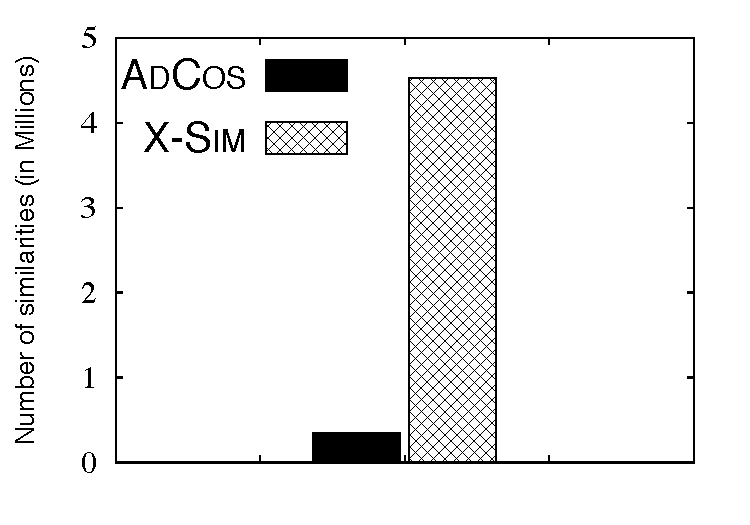
\includegraphics[height=1.6in,width=2.3in]{figures/Total_Sim.pdf}
\vspace{-6mm}
\caption{{\bf The number (millions) of inter-item similarities computed for the Amazon dataset using adjusted cosine similarity and \graphsim.}}
\label{fig:simCount}
\end{center}
\end{figure}

%\vspace{-2mm}
%\subsection{Baseline Similarity Graph}
\noindent{\bf Baseline Similarity Graph.} Our first step is to build the baseline similarity graph. There are several known methods for computing item-item similarities, e.g. Cosine, Pearson, Adjusted-cosine~\cite{sarwar2001item}. Though \graphsim can support any similarity metric as its baseline, we use adjusted-cosine which is shown to be more effective than the others~\cite{sarwar2001item}:
\begin{equation}
s_{ac}(i,j)=\frac{\sum _{u \in Y_i \cap Y_j} (r_{u,i} - \bar{r_u})(r_{u,j} - \bar{r_u})}{\sqrt{\sum _{u \in Y_i} (r_{u,i} - \bar{r_u})^2}\sqrt{\sum _{u \in Y_j} (r_{u,j} - \bar{r_u})^2}}
\label{adcos}
\end{equation}
In this first step, we compute the (baseline) similarities by integrating both $S$ and $T$ as a single domain. We denote by $G_{ac}$ the resulting similarity graph.\footnote{Here \emph{ac} denotes adjusted cosine.} We address the sparsity issue of $G_{ac}$ (Figure~\ref{fig:simCount}) by considering meta paths connecting both domains and then by extending $G_{a c}$. Clearly, a brute-force scheme considering all possible paths would be inefficient and not scalable. Assuming $m$ items in the database, the time complexity of such a brute-force scheme (computing path similarity for every pair of items) is $O(m^2)$, which is not suitable for big datasets like the Amazon one. \crossrec uses a layer-based pruning technique to consider only $O(k)$ paths for each item where $k \lll  m$. This pruning technique reduces the time complexity to $O(km) \simeq O(m)$.


\begin{figure}
\begin{center}
\includegraphics[height=1.8in,width=3.2in]{figures/dom_Cat.png}
\vspace{-2mm}
\caption{{\bf The layer-based pruning technique used in \crossrec.}}
\label{fig:domcat}
\end{center}
\end{figure}

%\vspace{-2mm}
%\subsection{X-Sim}
\noindent{\bf Layer-based Pruning.} Based on the baseline similarity graph, any item $i$ in a domain $D$ which connects to some item $j$ in another domain $D'$ is called a \emph{bridge item}. Both $i$ and $j$ are bridge items in this case. Any item that is not a bridge item is called a \emph{non-bridge item}. 

\crossrec's pruning technique partitions the items from $S$ and $T$ into six layers, as depicted in Figure~\ref{fig:domcat}. In turn, the items in each domain, say $D$, are divided into three layers (Figure~\ref{fig:domcat}).

\begin{itemize}
\item {\it BB-layer.} The (Bridge, Bridge)-layer consists of the bridge items of $D$ connected to the bridge items of another domain.

\item {\it NB-layer.} The (Non-bridge, Bridge)-layer consists of the non-bridge items of $D$ which are connected to bridge items of $D$.

\item {\it NN-layer.} The (Non-bridge, Non-bridge)-layer consists of the non-bridge items of $D$ which are not connected to other bridge items.
\end{itemize}

\crossrec then considers only the paths crossing different layers denoted by \emph{meta paths}.  Since a $k$-nearest neighbor method is used for the recommendation, \crossrec chooses, for each item $i$, the top-$k$ items from every neighboring layer. Let $G$ be the resulting top-$k$ similarity graph, which \crossrec treats as an undirected graph, i.e. if $i$ is one of $j$'s top-$k$ neighbors or $j$ is one of $i$'s top-$k$ neighbors then $i$ and $j$ are connected in $G$. Each node in $G$ has thus a degree at most $2k$. We describe the meta path selection via layers in more details in~\autoref{Implementation}.


\noindent{\bf \graphsim.} Consider any two items $i$ and $j$. We denote by $Y_{i \geq \bar{i}}$ the set of users who rated item $i$ higher than or equal to the average rating for $i$ over all the users in the database who rated it. We also denote by $Y_{i < \bar{i}}$ as the set of users who rated item $i$ lower than the average rating for $i$. Additionally, we denote by $n(Y_i)$ the cardinality of the set $Y_i$. 

\begin{definition}[Weighted Significance]
Given a pair of items $i$ and $j$, we define weighted significance ($S_{i,j}$) as the number of users who mutually agree or disagree on their preference for this pair. More precisely, we define the weighted significance ($S_{i,j}$) between $i$ and $j$ as follows.
$$
S_{i,j}= \underbrace{\left\vert{Y_{i \geq \bar{i}} \cap Y_{j \geq \bar{j}}}\right\vert}_\text{Mutual agreement} + \underbrace{\left\vert{Y_{i < \bar{i}} \cap Y_{j < \bar{j}}}\right\vert}_\text{Mutual disagreement}
$$
%$$
%S_{i,j}= \underbrace{n(Y_{i \geq \bar{i}} \cap Y_{j \geq \bar{j}})}_\text{Mutual agreement} + \underbrace{n(Y_{i < \bar{i}} \cap Y_{j < \bar{j}})}_\text{Mutual disagreement}
%$$
\end{definition}
Intuitively, higher significance value implies higher importance of the similarity value. For example, a similarity value of 0.5 between an item-pair ($i$,$j$) with $S_{i,j}=1000$ is more significant than a similarity value of 0.5 between an item-pair ($i$,$k$) with $S_{i,k}=1$ (for the latter may be a result of pure coincidence).

\begin{definition}[Meta Path]
Given $G$ and its six corresponding layers of items, we define a meta path as the path that contains at most one item from each layer.
\end{definition}
For every meta path $p = i_1 \leftrightarrow i_2 \ldots \leftrightarrow i_k$, we compute the path similarity $s_p$, weighted by its significance value, as follows.
\[ s_p = \frac{\sum_{t=1}^{t=k-1} S_{i_{t},i_{t+1}} \cdot s_{a c} (i_{t}, i_{t+1})}{\sum_{t=1}^{t=k-1}  S_{i_{t},i_{t+1}}}  \]
%\[ s_p = \frac{S_{i_1,i_2} \cdot s_{a c} (i_1, i_2) + \ldots + S_{i_{k-1},i_k} \cdot s_{a c} (i_{k - 1}, i_k)}{S_{i_1,i_2} + \ldots + S_{i_{k-1},i_k}} \]

For each pair of items $(i, j)$ from different domains, if $i$, $j$ are not connected directly, we aggregate the path similarities of all meta paths connecting $i$ and $j$. Due to the different lengths and similarities for paths, we have to give different weights to different paths. Shorter paths produce better similarities in recommenders~\cite{ramakrishnan2001privacy,sun2011pathsim} and hence are more preferred over longer ones. We now explain the strategy behind assigning these weights and thereby computing the \graphsim values.

\begin{definition}[Fractional Weighted Significance]
Given a pair of items $i$ and $j$, we define fractional weighted significance ($F_{i,j}$) between $i$ and $j$ as their significance value weighted by the inverse of number of users rating either $i$ or $j$. More precisely, we denote fractional weighted significance as follows. $$
F_{i,j}=\frac{S_{i,j}}{n(Y_i \cup Y_j)}
$$
\end{definition}

%We denote \emph{fractional mutuality} ($F_{i,j}$) between $i$ and $j$ as:

Next, we define the notion of \emph{path certainty} ($c_p$) of a meta path to take into account the factor of varying path lengths.
\begin{definition}[Path Certainty]
Given a meta path ($p = i_1 \leftrightarrow i_2 \ldots \leftrightarrow i_k$), we compute the path certainty ($c_p$) of the meta path $p$ as the product of the fractional weighted significance between each consecutive pair of items in the path $p$. More precisely, we define the path certainty as follows.
$$
c_p= \prod_{t=1}^{t=k-1} F_{i_{t}, i_{t+1}}
$$
%$$
%c_p= F_{i_1,i_2} \times \ldots \times F_{i_{k-1},i_k}
%$$ 
\end{definition}

Finally, we define our \graphsim metric as follows.

\begin{definition}[X-Sim]
Let $P (i, j)$ denote the set of all meta paths connecting items $i$ and $j$. We define the \graphsim for the item pair (i,j) as the path similarity weighted by the path certainty for all paths in $P(i,j)$. More precisely, we define \graphsim for any given pair of items $i$ and $j$ as follows.
$$
\textsc{X-Sim} (i, j) = \frac{\underset{p \in P (i, j)}{\sum} c_p \cdot s_p}{\underset{p
   \in P (i, j)}{\sum} c_p} 
$$
\end{definition}


%RGRG shouldn't this be a footnote?
Here, \graphsim{($i$,$j$)} denotes the heterogeneous similarity between any two items $i$ and $j$. Note that a trivial transitive closure over similarities would not take into account these factors, which would in turn impact the heterogeneous similarities and the recommendation quality.

\vspace{-2mm}
\section{Recommendation}
\label{Recommendation}
We show in this section how to leverage our \graphsim metric to generate artificial (AlterEgo) profiles of users in domains where the users might not have any activity yet. We present both a privacy-preserving (\crossrec) and a non-privacy-preserving (\npcrossrec) schemes.\footnote{Recall that \npcrossrec is used to demonstrate the effectiveness of \graphsim without the additional privacy overhead which can be useful for intra-company heterogeneous services like \emph{Amazon} or \emph{Google Play}.}  
% the recommendation computation scheme underlying both our \crossrec (as well as \npcrossrec\footnote{We denote a non-private version of \crossrec as \npcrossrec.}) which consists of the following four phases.

\subsection{Similarity Computation Phase}
We call the similarities computed in this phase as the \emph{baseline} similarities. For this phase, \crossrec treats both the source and target domains as a single domain and computes all pairwise item similarities. Basically, \crossrec computes the adjusted cosine similarities between the items in $I^S \cup I^T$ based on the preferences of the users in $U^S \cup U^T$ for these items. We distinguish two types of similarities which are as follows.

\noindent{\bf Homogeneous similarities.} These similarities are computed between items in the same domain. For instance, the similarity between a book and another one is homogeneous. Such similarities are used for intra-domain extension in \autoref{Implementation}.

\noindent{\bf Heterogeneous similarities.} These similarities are computed between items in different domains. For instance, the similarity between a book and a movie is heterogeneous. Such similarities are used for cross-domain extension in \autoref{Implementation}.

This phase remains the same for both \crossrec as well as \npcrossrec.


\subsection{{\large \bf \graphsim} Computation Phase}
After the computation of the baseline item-item similarities, \crossrec uses the \graphsim metric at first within a single domain to extend and improve the connections between the bridge items of a domain and other items within the same domain. Next, \crossrec uses the \graphsim metric to extend the similarities between items across the domains (which we explain in more details in~\autoref{Implementation}). At the completion of the heterogeneous similarity extension, for each item in source domain ($D^S$), there exists a corresponding set of items in target domain ($D^T$) with quantified (positive or negative) \graphsim values. This phase is the same for both \crossrec as well as \npcrossrec.

\subsection{AlterEgo Generation Phase}
In this phase, the profile of Alice (in $D^S$) is mapped to her AlterEgo profile (in $D^T$) as shown in Figure~\ref{fig:alterego}. For pedagogical reasons, we first present the non-private case followed by the private one.

%\subsubsection*{{\it \large\npcrossrec} AlterEgo generation}
\noindent{\bf \npcrossrec AlterEgo generation.} The non-private mapping is performed in two steps which are as follows.

{\it Similar item computation.} In this step, for every item $i$ in $D^S$, we determine the replacement item $j$ in $D^T$. Here, $j$ is the item which is most similar to $i$ based on the heterogeneous similarities computed using \graphsim.


{\it AlterEgo profile construction.} We then replace every item rated by Alice in $D^S$ with the most similar item in $D^T$ computed in the previous step. This item replacement induces the AlterEgo profile\footnote{If Alice has rated a few items in $D^T$ then the mapped profile is appended to her original profile in $D^T$ to build her AlterEgo profile.} of Alice in the target domain as shown in Figure~\ref{fig:alterego}.\\
This AlterEgo profile of Alice is the mapped profile of Alice from the source domain to the target domain.
\begin{figure}[!htb]
\begin{center}
\vspace{-7mm}
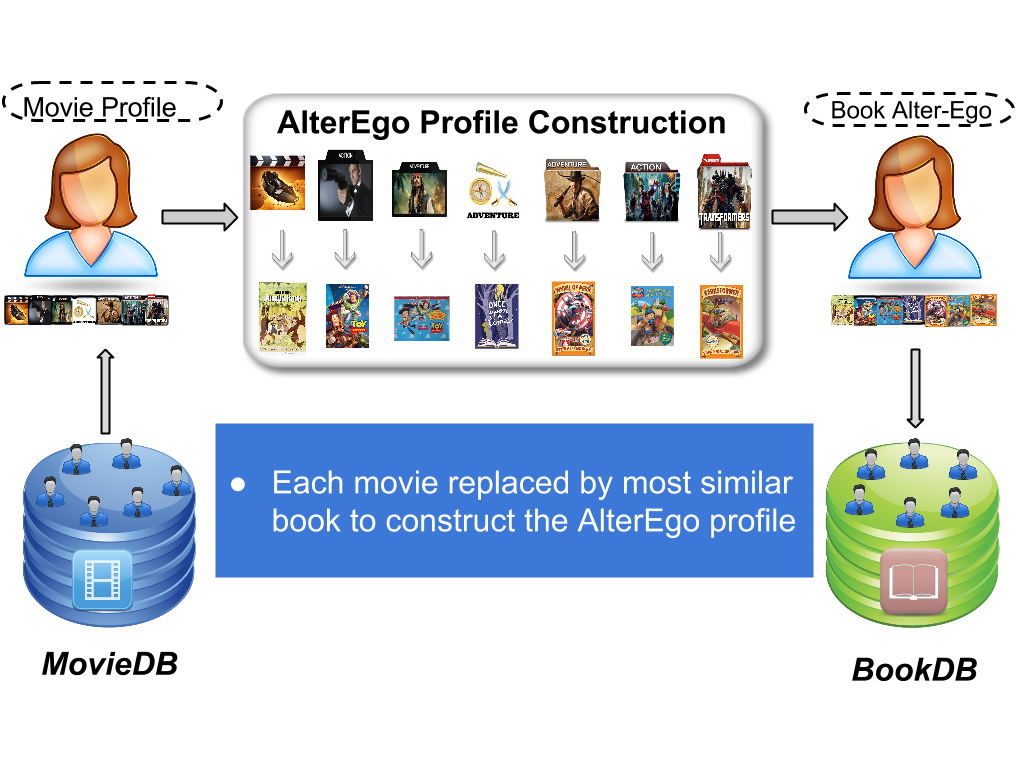
\includegraphics[height=2.5in,width=3.3in]{figures/AlterEgo.png}
\vspace{-12mm}
\caption{{\bf Alice's AlterEgo profile (in target domain) mapped from her original profile (in source domain).}}
\vspace{-2mm}
\label{fig:alterego}
\end{center}
\end{figure}

%\subsubsection*{{\it \large\crossrec} AlterEgo generation}

\noindent{\bf \crossrec AlterEgo generation.} The private mapping is performed in two steps which are as follows.

{\it Private replacement selection.} We consider Differential privacy~\cite{dwork2006calibrating} which is a technique for releasing statistical information about a database without revealing information about its individual entries. More specifically, differential privacy is defined as follows.


\begin{definition}[Differential Privacy~\cite{dwork2006calibrating}]
A randomized function $\mathcal{R}$ provides $\epsilon$-differential privacy if for all datasets $\mathcal{D}_1$ and $\mathcal{D}_2$, differing on at most one user profile, and all $t \in Range(\mathcal{R})$, the following inequality always holds:
$$\frac{Pr[\mathcal{R}(\mathcal{D}_{1} ) = t]}{Pr[\mathcal{R}(\mathcal{D}_{2}) = t]} \le exp(\epsilon)$$
\end{definition}


We leverage an exponential mechanism to design our differentially private replacement selection technique (Algorithm~\ref{Algo:prs}). The following theorem conveys our resulting privacy guarantee.

\begin{theorem}
Given an item $t_i$, the sensitivity of \graphsim is denoted by GS and the similarity between $t_i$ and any arbitrary item $t_j$ is denoted by $\graphsim(t_i,t_j)$. Then, the Private Replacement Selection (PRS) mechanism, which outputs $t_j$ as the replacement with a probability proportional to $exp(\frac{\epsilon \cdot \graphsim (t_i,t_j)}{2 \cdot GS})$, provides $\epsilon$-differential privacy.
\end{theorem}

\begin{proof}[sketch]
We now present a sketch of our proof. Consider two datasets $D$ and $D'$ which differ at one user, say $u$. We denote \graphsim($t_i$,$t_j$) in dataset D by $q(D,t_i,t_j)$ and the set of items in target domain, with quantified \graphsim values, by $I(t_i)$. Furthermore, $q(D,I(t_i))$ denotes the set of \graphsim values between $t_i$ and each item in $I(t_i)$. The global sensitivity (GS) is defined as $max_{D'}||q(D,t_i,t_j) - q(D',t_i,t_j)||_1$. Our PRS mechanism outputs an item $t_j$ as a private replacement for $t_i$. Then, we have the following:
\begin{flalign*}
 &
\frac{Pr[PRS(t_i, I(t_i), q(D,I(t_i)))= t_j]}{Pr[PRS(t_i, I(t_i), q(D',I(t_i)))= t_j]}& 
\end{flalign*}

\begin{flalign*}
 &= \frac{exp(\frac{\epsilon \cdot q(D,t_i,t_j)}{2 \cdot GS})}{\sum \limits_{t_k \in I(t_i)} exp(\frac{\epsilon \cdot q(D,t_i,t_k)}{2 \cdot GS})} \div \frac{exp(\frac{\epsilon \cdot q(D',t_i,t_j)}{2 \cdot GS})}{\sum \limits_{t_k \in I(t_i)} exp(\frac{\epsilon \cdot q(D',t_i,t_k)}{2 \cdot GS})} & 
\end{flalign*}


\begin{flalign*}
 &= \underbrace{\frac{exp(\frac{\epsilon \cdot q(D,t_i,t_j)}{2 \cdot GS})}{exp(\frac{\epsilon \cdot q(D',t_i,t_j)}{2 \cdot GS})}}_\text{P} \cdot \underbrace{\frac{\sum \limits_{t_k \in I(t_i)} exp(\frac{\epsilon \cdot q(D',t_i,t_k)}{2 \cdot GS})}{\sum \limits_{t_k \in I(t_i)} exp(\frac{\epsilon \cdot q(D,t_i,t_k)}{2 \cdot GS})}}_\text{Q}&
\end{flalign*}

\begin{flalign*}
&P= exp(\frac{\epsilon \cdot (q(D,t_i,t_j) -q(D',t_i,t_j))}{2 \cdot GS}) \le exp(\frac{\epsilon}{2})&
\end{flalign*}

\begin{flalign*}
&Q= \frac{\sum \limits_{t_k \in I(t_i)} exp(\frac{\epsilon \cdot q(D',t_i,t_k)}{2 \cdot GS})}{\sum \limits_{t_k \in I(t_i)} exp(\frac{\epsilon \cdot q(D,t_i,t_k)}{2 \cdot GS})} \le exp(\frac{\epsilon}{2})&
\end{flalign*}

Therefore, we have:
$$
\frac{Pr[PRS(t_i, I(t_i), q(D,I(t_i)))= t_j]}{Pr[PRS(t_i, I(t_i), q(D',I(t_i)))= t_j]} \le exp(\epsilon)
$$
Hence, PRS provides $\epsilon$-differential privacy.
\end{proof}
%The detailed proof is available in our companion technical report for interested readers~\cite{}.


%In~\cite{zhu2013differential,zhu2014effective}, the authors proposed a private neighbor selection mechanism which can provide high quality neighbors and gurantees differential privacy simultaneously. Inspired by this mechanism, we compute the private replacement for the actual item leveraging the exponential mechanism as shown in Algorithm~\ref{Algo:prs}.

\begin{algorithm}[!htb]
\caption{\small\itshape Private Replacement Selection Algorithm: \quad \quad PRS($t_i$,I($t_i$),\emph{X-Sim}(I($t_i$))) where I($t_i$) is the set of items in the target domain with \graphsim values.}
\label{Algo:prs}
\begin{algorithmic}[1]
\Require $\epsilon, t_i, I(t_i), \emph{X-Sim}(I(t_i))$		\hfill $\rhd$ $\epsilon:$ Privacy parameter
\State Global sensitivity for \graphsim:\\ GS= $|\graphsim_{max} - \graphsim_{min}|$=2

\For  {item $t_j$ in $I(t_i)$}
\State Allocate probability as:
\vspace{-3mm}
$$
\frac{exp(\frac{\epsilon \cdot \graphsim (t_i,t_j)}{2 \cdot GS})}{\sum \limits_{t_k \in I(t_i)} exp(\frac{\epsilon \cdot \graphsim (t_i,t_k)}{2 \cdot GS})}
$$
\vspace{-4mm}
\EndFor


\State Sample an element $t$ from $I(t_i)$ according to their probability.
\State Return $t$; \hfill $\rhd$ $\epsilon$-differentially private replacement for $t_i$
\end{algorithmic}
\end{algorithm}


{\it AlterEgo profile construction.} In this step, we replace every item rated by Alice in $D^S$ with the item in $D^T$ returned by the private mechanism in the previous step. This item replacement leads to an AlterEgo profile of Alice in the target domain.

Note that this private AlterEgo profile protects the privacy of the straddlers, users who rated in both the domains, as the ratings of these users are used to compute the heterogeneous similarities leaving their privacy at risk~\cite{ramakrishnan2001privacy}. In addition, if the domains are typically two different applications owned by different companies like Netflix and Last.fm, then this mechanism aids the exchange of AlterEgo profiles while preventing curious or malicious users to infer about the preferences of others. 



%Additionally, this privacy mechanism also facilitates the exchange of AlterEgo profiles without releasing private information about their customers. Note that there are ways to compute the heterogeneous cosine similarities using secure protocols based on zero-knowledge proofs~\cite{yang2013secure,kikuchi2010privacy,zhang2014secure,wong2013privacy} and the homogeneous item similarties can be released in a differential private manner~\cite{mcsherry2009differentially} but this is out of the scope of this paper.  



\subsection{Recommendation Phase}
We now present the recommendation computation steps. Again, we first explain the non-private case followed by the private one.

%\subsubsection*{{\it \large\npcrossrec} recommendation} leveraging the notion of \emph{temporal collaborative filtering}~\cite{liu2010online, ding2005time}
\noindent{\bf \npcrossrec recommendation.} The AlterEgo profile of Alice is used along with the original profiles in the target domain to compute the top-k similar users for Alice and then compute recommendations for Alice leveraging the profiles of the $k$ most similar users from the target domain using Algorithm \ref{ub_cf}. The item-based version of \crossrec leverages this AlterEgo profile and computes the recommendations as demonstrated in Algorithm \ref{ib_cf}. For the item-based version of \crossrec, we improve the recommendation quality further by adding a time-based weight to the ratings. The predictions (Equation~\ref{pred_ib_cf}), weighted by the time-based parameter ($\alpha$), for the ratings are computed as follows.
\begin{equation}
\label{pred_ib_cf_time}
Pred[i] (t)=\bar{r}_{i} +\frac{\sum_{j \in N_{i}} \tau(i,j) \cdot (r_{A,j}- \bar{r}_j) \cdot e^{-\alpha (t-t_{A,j})}}{\sum_{j \in N_{i}} |\tau(i,j)| \cdot e^{-\alpha (t-t_{A,j})} } 
\end{equation}
Note that the prediction has a time-based relevance factor ($e^{-\alpha (t-t_{A,j})}$) with decaying rate controlled by parameter $\alpha$ to determine each rating's weight for the prediction computation. Here, $t_{A,j}$ denotes the \emph{timestep}\footnote{The timestep is a logical time corresponding to the actual timestamp of an event.} when user $A$ rated item $j$. The time-based CF feature is applicable to the item-based CF approach as the prediction computation (Equation~\ref{pred_ib_cf_time}) for a user $A$ is dependent only on her previous ratings for similar items and thereby leverages time as observed by $A$.

%\subsubsection*{{\it \large\crossrec} recommendation}
\noindent{\bf \crossrec recommendation.} 
The private AlterEgo profile of Alice is used along with the original profiles in the target domain to compute the recommendations for Alice. To demonstrate the flexibility of our heterogeneous recommender, the recommendation step is integrated with a differential private approach, inspired by Zhu et al.~\cite{zhu2013differential,zhu2014effective}, to protect users in the target domain against other curious users. We implemented both item-based and user-based versions of \crossrec. The item-based recommendation mechanism is demonstrated in Algorithm~\ref{PrivRecoAlgo} which leverages the PNSA mechanism (Algorithm~\ref{Algo:pnsa}). We now present our modified recommendation-aware sensitivity along with its correctness proof sketch.\footnote{Our notion of recommendation-aware sensitivity is slightly different from the one presented in~\cite{zhu2013differential,zhu2014effective}.}

\begin{definition}[Local Sensitivity]
For a given function $f: \mathcal{R} \rightarrow R$ and a dataset $D$, the Local Sensitivity of $f$ is defined as $LS_f = \max \limits_{D'}\Arrowvert f(D) - f(D')\Arrowvert_1$, where $D$ and $D'$ are neighboring datasets which differ at one user profile. 
\end{definition}


We define a rating vector $r_{t_i} = \lbrack r_{t_{ai}}, ..., r_{t_{xi}}, r_{t_{yi}} \rbrack$ which consists of all the ratings for an item $t_i$ in the dataset $D$. Similarly, we have a rating vector $r'_{t_i}$ for $t_i$ in the neighboring dataset $D'$. Since we use adjusted-cosine for \graphsim, a rating $r_{t_{xi}}$ is the result after subtracting the average rating of user $x$ ($\bar{r}_x$) from the actual rating provide by $x$ for an item $i$. The recommendation-aware sensitivity is defined as follows.

\begin{theorem}[Recommendation-aware sensitivity]
\begin{sloppypar}
Given a score function $q: \mathcal{R} \rightarrow R$ and a dataset $D$, we define the recommendation-aware sensitivity corresponding to a score function $q_i(I,t_j)$ for a pair of items $t_i$ and $t_j$ as:
\end{sloppypar}
\begin{flalign*}
&RS(t_i, t_j) = max \{ max_{u_x \in U_{ij}} (\frac{r_{t_{xi}} \times r_{t_{xj}}}{\parallel r'_{t_i} \parallel \times \parallel r'_{t_j} \parallel}),&
\end{flalign*}

\begin{flalign*}
 max_{u_x \in U_{ij}} (\frac{r_{t_i} \cdot r_{t_j}} {\parallel r'_{t_i} \parallel \times \parallel r'_{t_j} \parallel} - \frac{r_{t_i} \cdot r_{t_j}} {\parallel r_{t_i} \parallel \times \parallel r_{t_j} \parallel})\} &
\end{flalign*}
\end{theorem}

\begin{proof}[sketch]
\begin{sloppypar}
We now provide a proof sketch of the recommendation-aware sensitivity which is measured by the maximal change in the similarity between two items when deleting a user's rating. The score function ($q$) for a pair of items $t_i$ and $t_j$ is defined as their similarity value ($s(t_i, t_j)$). First, we have:
\end{sloppypar}
\begin{align*}
RS(t_i, t_j) &= 
max \parallel s(t_i, t_j) - s'(t_i, t_j)\parallel_1
\end{align*}

After inserting the similarity values for $s(t_i, t_j)$, we have:
\begin{flalign*}
& s(t_i, t_j) - s'(t_i, t_j) = \frac{r_{t_i} \cdot r_{t_j}}{\parallel r_{t_i} \parallel \times \parallel r_{t_j} \parallel} - 
\frac{r'_{t_i} \cdot r'_{t_j}}{\parallel r'_{t_i} \parallel \times \parallel r'_{t_j} \parallel} &
\end{flalign*}

\begin{flalign*}
& =\frac{r_{t_i} \cdot r_{t_j} \times \parallel r'_{t_i} \parallel \times \parallel r'_{t_j} \parallel -
r'_{t_i} \cdot r'_{t_j} \times \parallel r_{t_i} \parallel \times \parallel r_{t_j} \parallel 
}{\parallel r_{t_i} \parallel \times \parallel r_{t_j} \parallel \times \parallel r'_{t_i} \parallel \times \parallel r'_{t_j} \parallel}=\frac{P}{Q} &
\end{flalign*}

We assume that the profile of a user $x$, in $D$, is not present in $D'$. This user rated both $t_i$ and $t_j$. Note that if this user rated one of these items or none, then the similarity value does not depend on the presence or absence of this user in the dataset. We have: $\parallel r'_{t_i} \parallel \times \parallel r'_{t_j} \parallel \leq \parallel r_{t_i} \parallel \times \parallel r_{t_j} \parallel$. 

We have P= ($r_{t_i} \cdot r_{t_j} \times \parallel r'_{t_i} \parallel \times \parallel r'_{t_j} \parallel -
r'_{t_i} \cdot r'_{t_j} \times \parallel r_{t_i} \parallel \times \parallel r_{t_j} \parallel$) and Q=($\parallel r_{t_i} \parallel \times \parallel r_{t_j} \parallel \times \parallel r'_{t_i} \parallel \times \parallel r'_{t_j} \parallel$).
Since $Q \geq 0$, we have two conditions depending on whether $P \geq 0$ or $P \leq 0$.

If $P \geq 0$, then 
\begin{flalign*}
&\parallel s(t_i, t_j) - s'(t_i, t_j) \parallel_1 \leq \frac{(r_{t_i} \cdot r_{t_j} - r'_{t_i} \cdot r'_{t_j})}
{\parallel r'_{t_i} \parallel \times \parallel r'_{t_j} \parallel}= \frac{r_{t_{xi}} \times r_{t_{xj}}}{\parallel r'_{t_i} \parallel \times \parallel r'_{t_j} \parallel}.&
\end{flalign*}

If $P \leq 0$, then 
\begin{flalign*}
& \parallel s(t_i, t_j) - s'(t_i, t_j) \parallel_1 \leq \frac{r_{t_i} \cdot r_{t_j}} {\parallel r'_{t_i} \parallel \times \parallel r'_{t_j} \parallel} - \frac{r_{t_i} \cdot r_{t_j}} {\parallel r_{t_i} \parallel \times \parallel r_{t_j} \parallel}.&
\end{flalign*}

Hence, we have the recommendation-aware sensitivity as:
\begin{flalign*}
&RS(t_i, t_j) = max \{ max_{u_x \in U_{ij}} (\frac{r_{t_{xi}} \times r_{t_{xj}}}{\parallel r'_{t_i} \parallel \times \parallel r'_{t_j} \parallel}),&
\end{flalign*}

\begin{flalign*}
 max_{u_x \in U_{ij}} (\frac{r_{t_i} \cdot r_{t_j}} {\parallel r'_{t_i} \parallel \times \parallel r'_{t_j} \parallel} - \frac{r_{t_i} \cdot r_{t_j}} {\parallel r_{t_i} \parallel \times \parallel r_{t_j} \parallel})\} &
\end{flalign*}
\end{proof}
%The detailed proof is available in our companion technical report for interested readers~\cite{}.


%(Our correctness proof is available in~\autoref{sensitivity}). 
%In the following, we revisit the two theorems, presented in~\cite{zhu2013differential,zhu2014effective}, which prove that this truncated similarity can enhance the quality of neighbors.
Similar to \cite{zhu2013differential,zhu2014effective}, we use a \emph{truncated similarity} (Step 7 in Algorithm~\ref{Algo:pnsa}) along with our revised recommendation-aware sensitivity to enhance the quality of selected neighbors. The two theorems which prove that this truncated similarity along with our recommendation-aware sensitivity can enhance the quality of neighbors are as follows. (The proofs have been omitted due to lack of space.)%\footnote{The proofs are presented in our companion technical report for interested readers~\cite{}.})


% and follow the same methodology as in~\cite{zhu2013differential,zhu2014effective}

\begin{theorem}
\label{theorem_1}
Given an item $t_i$, we denote its $k$ neighbors by $N_k(t_i)$, the maximal length of all the rating vector pairs by $|v|$, the minimal similarity among the items in $N_k(t_i)$ by $Sim_k(t_i)$ and the maximal recommendation-aware sensitivity between $t_i$ and other items by RS. Then, for a small constant  $0< \rho <1$, the similarity of all the items in $N_k(t_i)$ are larger than $(Sim_k(t_i) -w)$ with a probability at least $1 - \rho$, where $w=min(Sim_k(t_i), \frac{4k \times RS}{\epsilon'} \times ln\frac{k \times (|v| - k)}{\rho})$.
\end{theorem}

Intuitively, Theorem~\ref{theorem_1} implies that the selected neighbors have similarities greater than some threshold value $(Sim_k(t_i) -w)$ with a high probability ($1 - \rho$).

\begin{theorem}
\label{theorem_2}
Given an item $t_i$, for a small constant   $0 <\rho <1$, all items with similarities greater than $(Sim_k(t_i) +w)$ are present in $N_k(t_i)$ with a probability at least $1-\rho$ where $w=min(Sim_k(t_i), \frac{4k \times RS}{\epsilon'} \times ln\frac{k \times (|v| - k)}{\rho})$.
\end{theorem}

Intuitively, Theorem~\ref{theorem_2} implies that the items with similarities greater than some threshold value $(Sim_k(t_i) +w)$ are selected as neighbors with a high probability ($1 - \rho$).

Both theorems prove that the truncated similarity along with our recommendation-aware sensitivity provides good quality of neighbors while providing $\epsilon'/2$-differential privacy. The predictions are finally computed leveraging the PNCF mechanism (Algorithm~\ref{PrivRecoAlgo}) which adds Laplacian noise to provide $\epsilon'/2$-differential privacy. By additive property of differential privacy, PNSA and PNCF together provides $\epsilon'$-differential privacy. The item-based version of \crossrec includes the additional feature of \emph{time-based relevant} predictions to boost the recommendation quality traded for privacy.

Here we provide only one demonstration of the flexibility of our heterogeneous recommender due to lack of space. Since the AlterEgo profile can be considered as an actual profile in the target domain, thereby any homogeneous recommendation algorithm~\cite{adomavicius2005toward} like Matrix Factorization techniques, can be applied to the target domain to generate the recommendations.


\begin{algorithm}[!htb]
\caption{\small\itshape Private Neighbor Selection : PNSA($t_i$,I,\emph{Sim}($t_i$)) where $I$ is the set of all items.}
\label{Algo:pnsa}
\begin{algorithmic}[1]
\Require $\epsilon', w, t_i, I, \emph{Sim}(t_i)$, k		\hfill $\rhd$ $\epsilon':$ Privacy 
    \State $C_1 = \lbrack t_j | s(t_i, t_j) \geq \emph{Sim}_k(t_i)-w, t_j \in I\rbrack$
    \State $C_0 = \lbrack t_j | s(t_i, t_j) < \emph{Sim}_k(t_i)-w, t_j \in I\rbrack$
    \State $w=min(\emph{Sim}_k(t_i), \frac{4k \times RS}{\epsilon'} \times ln\frac{k \times (|v| - k)}{\rho})$
	\For  {N=1:k}
    \For  {item $t_j$ in $I$}
    \State \vspace{-6mm} {\small
        \begin{flalign*}
        RS(t_i, t_j)= max \{
        max_{u_x \in U_{ij}} (\frac{r_{t_{xi}} \times r_{t_{xj}}}{\parallel r'_{t_i} \parallel \times \parallel r'_{t_j} \parallel}),\\ 
        max_{u_x \in U_{ij}} (\frac{r_{t_i} \cdot r_{t_j}} {\parallel r'_{t_i} \parallel \times \parallel r'_{t_j} \parallel} - \frac{r_{t_i} \cdot r_{t_j}} {\parallel r_{t_i} \parallel \times \parallel r_{t_j} \parallel)}
        )\}
        \end{flalign*}}\vspace{-4mm}
    \State $\widehat{\emph{Sim}}(t_i, t_j) = max(\emph{Sim}(t_i, t_j), \emph{Sim}_k(t_i) - w)$
    \State Allocate probability as:\hfill $\rhd$ $\frac{\color{red}\epsilon'}{\color{red}2k}$-Privacy
    \vspace{-3mm}
    $$
    \frac{exp(\frac{{\color{red} \epsilon'} \cdot \widehat{\emph{Sim}}(t_i, t_j)}{{\color{red} 2k} \times 2RS(t_i, t_j)})}{\sum \limits_{l \in C_1} exp(\frac{ {\color{red} \epsilon'} \cdot \widehat{\emph{Sim}}(t_i, t_l)}{{\color{red} 2k} \times 2RS(t_i, t_l)}) +  \sum \limits_{l \in C_0} exp(\frac{{\color{red} \epsilon'} \cdot \widehat{\emph{Sim}}(t_i, t_l)}{{\color{red} 2k} \times 2RS(t_i, t_l)})}
	$$
    \vspace{-4mm}
	\EndFor 

	\State Sample an element $t$ from $C_1$ and $C_0$ without replacement according to their probability.
	\State $N_k(t_i)=N_k(t_i) \cup t$
	\EndFor
	\State Return $N_k(t_i)$; 
\end{algorithmic}
\end{algorithm}


\begin{algorithm}[!htb]
\caption{\small\itshape Private Recommendation: PNCF($P_A, I$) \quad \quad where $P_A$ denotes the AlterEgo profile of Alice, and $I$ denotes the set of all items.}
\label{PrivRecoAlgo}
\begin{algorithmic}[1]
\State var P; \hfill $\rhd$ Dictionary with predictions for Alice
\State var $\tau$; \hfill $\rhd$ User similarities
\State var $\bar{r}$; \hfill $\rhd$ Average rating for each items
\State var $\epsilon'$ \hfill $\rhd$ Degree of privacy
\State var $N_k$ \hfill $\rhd$ Private neighbors using PNSA
\For {$t_i$ : $item$ in $P_A$}
\For {$t_j$ : $item$ in $N_k(t_i)$}
\State \hspace{-5mm}$P[t_j]=\bar{r}_{t_j} +\frac{\sum_{t_k \in N_k(t_j)} (\tau(t_k, t_j) + Lap(\frac{RS(t_k, t_j)}{\epsilon' / 2})) \cdot (r_{A,t_k}- \bar{r}_{t_k})}{\sum_{t_k \in N_k(t_j)} |\tau(t_k, t_j) + Lap(\frac{RS(t_k, t_j)}{\epsilon' / 2})| }$
\EndFor
\EndFor

\State $R_{A}=P.sortByValue(ascending=false);$
\State \textbf{return:} $R_{A}[:N]$; \hfill $\rhd$ Top-N recommendations for Alice
\end{algorithmic}
\end{algorithm}


\iffalse
\For {$C$ : $user$ in $N_A$}
\State $\tau_{n}(A, C) = \tau(A, C) + Lap(\frac{RS(A, C)}{\epsilon' / 2});$\hfill $\rhd \epsilon':$ Privacy
\EndFor
\For {$i$ : $item$ in $I$}
\State $Pred[i]=\bar{r}_{A} +\frac{\sum_{B \in N_{A}} \tau_{n}(A,B) \cdot (r_{B,i}- \bar{r}_B)}{\sum_{B \in N_{A}} |\tau_{n}(A,B)| } ;$
\EndFor
\fi
\vspace{-2mm}
\section{Implementation}
\label{Implementation}
In this section, we describe our implementation of \crossrec (as well as \npcrossrec). Figure~\ref{fig:XMap_Arch} outlines the four main components of our implementation: \emph{baseliner}, \emph{extender}, \emph{generator} and \emph{recommender}. We describe each of these components along with their functionality. Note that only the baseliner component remains same for \crossrec and \npcrossrec.

\begin{figure}
\begin{center}
\includegraphics[height=1.8in,width=3.4in]{figures/X-Frame.png}
\caption{{\bf The components of \crossrec: \emph{Baseliner, Extender, Generator, Recommender}.}}
\vspace{-3mm}
\label{fig:XMap_Arch}
\end{center}
\end{figure}

%\subsection{Preprocessor}
%The preprocessor partitions the data into \emph{training} and \emph{test} sets. The training set is used to build up the item-item network in \crossrec whereas the test set is used to evaluate the quality of the prediction provided by \crossrec.

\subsection{Baseliner}
The Baseliner computes the baseline similarities leveraging the adjusted cosine similarity (Equation~\ref{tau_ib_cf}) between the items in the two domains. It splits the item-pairs based on whether both the items belong to the same domain or not. If both items are from same domain, then the item-pair similarities will be delivered as \emph{homogeneous similarities}. If one of the items belongs to a different domain, then the item-pair similarities will be delivered as \emph{heterogeneous similarities}. The baseline heterogeneous similarities are computed based on the user overlap.\footnote{These are the baseline similarities without any extension or enhancements.}

\subsection{Extender}
This component extends the baseline similarities both within a domain and across domains. The items in each domain are divided into three layers based on our layer-based pruning technique as shown in Figure~\ref{fig:domcat}.
For every specific layer of items, the extender computes the top-k for the neighboring layers. For instance, for the items in the BB-layer of $D^S$, the extender computes the top-k from items in the BB-layer in $D^T$ and also the top-k from the items in the NB-layer in $D^S$. 
%Similarly, for the items in the NB-layer of $D^S$, the extender computes the top-k from the items in the BB-layer in $D^S$ and also the top-k from the items in the NN-layer in $D^S$. Finally, for the items in the NN-layer of $D^S$, the extender computes the top-k from the items in the NB-layer in $D^S$. We perform similar computations for the items in domain $D^T$.

\noindent{\bf Intra-domain extension.} In this step, the extender computes the \graphsim similarity for the items in the NN-layer in $D^S$ and the items in the BB-layer of $D^S$ via the NB-layer items of $D^S$. Similar computations are performed for the domain $D^T$.

\noindent{\bf Cross-domain extension.} After the previous step, the extender updates the NB and NN layers in both domains based on the new connections (top-$k$). Then, it updates the connections between the NB and BB layer items in one domain to the NB and BB category items in the other one.

At the end of the execution of the extender, for every item $t_i$ in $D_S$, we get a set of items $I(t_i)$ in $D_T$ with some quantified (positive or negative) \graphsim values with $t_i$. 

\subsection{Generator}
The generator performs the following two computational steps.

\noindent{\bf Item mapping.} The Generator maps every item in one domain (say $D^S$) to its most similar item (for \npcrossrec) or its private replacement (for \crossrec) in the other domain ($D^T$). After, the completion of this step, every item in one domain has a replacement item in the other domain.\footnote{Note that to have more diversity, we could also choose a set of replacements for an item in the target domain, based on the \graphsim metric. This however is out of the scope of this paper.}

\noindent{\bf Mapped user profiles.} The Generator here creates an artificial profile (AlterEgo) of a user in a target domain $D_T$ from her actual profile in the source domain $D_S$ by replacing each item in her profile in $D^S$ with its replacement in $D^T$ as shown in Figure~\ref{fig:alterego}.  Finally, after this step, the Generator outputs the AlterEgo profile of a user in the target domain where she might have little or no activity yet.

\subsection{Recommender}
This component leverages this artificial AlterEgo profile created by the the Generator to perform the recommendation computation. It can implement any general recommendation algorithm for its underlying recommendation computation. In this paper, we implemented user-based and item-based CF schemes. For \npcrossrec, the recommender uses Algorithm~\ref{ub_cf} (user-based CF) or Algorithm~\ref{ib_cf} (item-based CF) in the target domain. For \crossrec, the recommender also uses the PNSA algorithm along with the PNCF algorithm to generate recommendations either in a user-based manner or in an item-based manner. Additionally, for both \npcrossrec and \crossrec, the item-based CF recommender leverages the temporal relevance to boost the recommendation quality.{\color{red}TALK ABOUT MF!}


\section{Experimental Evaluation}
\label{Evaluation}
In this section, we report on our empirical evaluation of \crossrec on a cluster computing framework namely Spark with real world traces from Amazon~\cite{mcauley2013hidden} to analyze its prediction accuracy, privacy and scalability. We choose Spark as our cluster computing framework since the underlying framework to support \crossrec must be scalable and fault-tolerant.


\subsection{Experimental Setup}

\noindent{\bf Experimental platform.}
We perform all the experiments on a cluster consisting of 20 machines. Each machine is an Intel Xeon CPU E5520 @2.26GHz with 32 GB memory and 600 GB disk storage. The machines are connected through a 2xGigabit Ethernet (Broadcom NetXtremeII BCM5716).

\noindent{\bf Datasets.}
We use two sets of real traces from Amazon datasets~\cite{mcauley2013hidden}: \emph{movies} and \emph{books}. We use the ratings for the period from 2011 till 2013. The movies dataset consists of 743,735 ratings from 777,729 users for 168,105 movies where each user rated at least 10 movies. The books dataset consists of 1,424,135 ratings from 1,232,135 users for 567,731 books where each user rated at least 10 books. The ratings vary from 1 to 5 with an increment of 1 between the possible ratings. The overlapping users in these two datasets are those Amazon users who are present in both and are ascertained using their Amazon user-ids.
%From this original traces, we create two additional traces for our experiments. These dataset consists of users who rated at least 5 items in one domain. For users who rated in both the domains, these users also rated at least 10 items (5 from each domain). 

\noindent{\bf Evaluation metrics.}
We evaluate \crossrec along three complementary metrics: the recommendation \emph{quality} as perceived by the users in terms of prediction \emph{accuracy}, the degree of \emph{privacy} provided to the end-users in terms of the privacy parameters ($\epsilon, \epsilon'$) and the \emph{scalability} in terms of \emph{speedup} achieved in \crossrec by increasing the number of machines in the cluster.

{\it Accuracy.} We evaluate the accuracy of the predictions in terms of Mean Absolute Error (MAE). MAE computes the average absolute deviation between a predicted rating and the user's true rating. MAE is a standard metric used to evaluate state-of-the-art recommenders~\cite{breese1998empirical, herlocker1999algorithmic, shardanand1995social}. We assume that the predicted rating for an item $i$ is denoted by $p_i$ and the actual rating is denoted by $r_i$ in the test dataset. Then, the MAE for a test dataset, with $\mathcal{N}$ ratings, is computed as: $\frac{\sum _{i=1}^{\mathcal{N}}|p_i -r_i|}{\mathcal{N}}$. Given that $r_{min}$ and $r_{max}$ denotes the minimum and maximum ratings respectively, the following inequality always holds: $0< MAE < (r_{max}-r_{min})$. The lower the MAE, the more accurate the predictions.

%$$
%MAE=  \frac{\sum _{i=1}^{\mathcal{N}}|p_i -r_i|}{\mathcal{N}}
%$$  
%The lower the MAE, the more accurate the predictions.

{\it Privacy.} 
Our differential privacy guarantees are parameterized by the privacy parameters: $\epsilon$ for the Private Replacement Selection technique used for AlterEgo generation and $\epsilon'$ for the PNCF used for the private recommendation generation in \crossrec. According to the privacy literature~\cite{dwork2011firm, zhu2013differential,zhu2014effective}, $\epsilon=1$ or less would be suitable for privacy preserving purposes.

{\it Speedup.} We evaluate the speedup in terms of the time required for sequential execution ($T_1$) and the time required for parallel execution with $p$ processors ($T_p$). Amdahl's law~\cite{krishnaprasad2001uses} models the performance of speedup ($S_p$) as follows.
$$
S_p= \frac{T_1}{T_p}
$$
Due to the considerable size of the Amazon dataset, we compare the speedup on $p$ processors with respect to a minimum of $5$ processors ($T_5$) instead of a sequential execution ($T_1$).

\noindent{\bf Competitors.}
%The two systems (the two papers) which are used to compare with our system \crossrec along with the baseline approaches
We now present the recommenders against which we compare \crossrec. Existing recommendation schemes over several domains can be classified as follows.

{\it Linked-domain personalization.} The goal here is to recommend items in the target domain ($\mathcal{D}^T$) by exploring rating preferences aggregated from both source and target domains, i.e, to recommend items in $\mathcal{I}^T$ to users in $\mathcal{U}^S$ based on the preferences of users in $\mathcal{U}^S\; \cup \;\mathcal{U}^T$ for items in $\mathcal{I}^S \;\cup \;\mathcal{I}^T$. In this approach, ratings from multiple domains are aggregated into a single domain. Then, a traditional CF mechanism is applied over this aggregated single domain~\cite{sarwar2001item, cremonesi2011cross}. \textsc{Item-based-kNN} is a linked-domain personalization approach~\cite{sarwar2001item, cremonesi2011cross} where we use item-based collaborative filtering over the aggregated ratings over both the domains.

{\it Heterogeneous personalization.} The goal here is to recommend items in $\mathcal{I}^T$ to users in $\mathcal{U}^S$ based on the preferences of $\mathcal{U}^S$ for $\mathcal{I}^S$, $\mathcal{U}^T$ for $\mathcal{I}^T$ and $\mathcal{U}^S\; \cap\; \mathcal{U}^T$ for $\mathcal{I}^S\; \cup\; \mathcal{I}^T$. In this approach, the user similarities are first computed in both source and target domains. These domain-related similarities are then aggregated into the overall heterogeneous similarities. Finally, the $k$-nearest neighbors, used for recommendation computations, are selected based on these heterogeneous similarities~\cite{berkovsky2007cross}. In the \textsc{RemoteUser} approach~\cite{berkovsky2007cross}, the user similarities in source domain are used to compute the $k$ nearest neighbors for users who have not rated in target domain. Then user-based collaborative filtering is performed.

{\it Baseline prediction.} For sparse dataset, the baseline is provided by item-based average ratings~\cite{baltrunas2009context} or user-based average ratings~\cite{lemire2005slope}. The goal here is to predict based on the average ratings provided by users in $\mathcal{U}^S\; \cup\; \mathcal{U}^T$ for items in $\mathcal{I}^S\; \cup\; \mathcal{I}^T$. One of the most basic prediction scheme is the \textsc{ItemAverage} scheme where we predict that each item will be rated as the average over all users who rated that item~\cite{baltrunas2009context}. Note that though this technique gives a very good prediction of the actual rating but its not personalized.% and hence not suited for recommendation purpose.

We compare \crossrec with these three other systems namely: \textsc{Item-based-kNN}, \textsc{RemoteUser} and \textsc{ItemAverage}.

\noindent{\bf Evaluation scheme.} We partition the set of common users who rated both movies and books into \emph{training} and \emph{test} sets. For the test users, we hide their profile in the target domain (say books) and use their profile in the source domain (movies) to predict books for them. This strategy evaluates the accuracy of the predictions if the user did not rate any item in the target domain. Hence, we can evaluate the performance of \crossrec in the scenario where the test users did not rate any item in the target domain (cold-start). Additionally, if we hide part of the user profile in the target domain, then we can evaluate how \crossrec handles the scenario where the test users rated very few items in the target domain (sparsity). Furthermore, we denote the item-based variant of \crossrec as \crossrecib and the user-based variant as \crossrecub. Similarity for \npcrossrec, we denote the item-based variant of \npcrossrec as \npcrossrecib and the user-based variant as \npcrossrecub.
\subsection{Temporal Relevance}
In this section, we observe the temporal relevance effect for \crossrec, leveraging the item-based recommender, and then tune the temporal relevance parameter $\alpha$ accordingly. Figure~\ref{fig:temporal} demonstrates this effect compared to the approach without any temporal relevance effect ($\alpha=0$). We vary $\alpha$ between 0.01 to 0.3. Note that an item-based CF approach computes the predictions leveraging the target user's very few observed ratings on the nearest neighbors and given the very limited size of this set of ratings, any further amplification of $\alpha$ impacts predictions negatively as it reduces the contribution of old ratings furthermore. Hence, we set $\alpha$ for our experiments, based on Figure~\ref{fig:temporal}, to achieve optimal recommendation quality.% which guarantees better quality in all the four scenarios.
\begin{figure}
\begin{center}
\hspace{-3mm}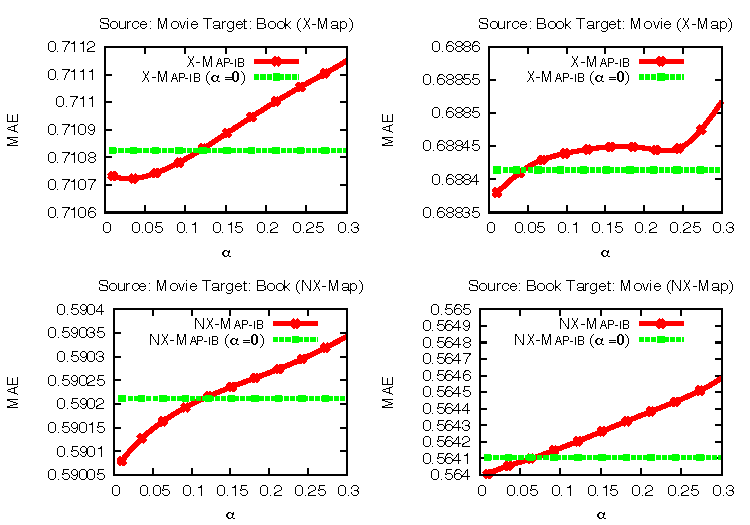
\includegraphics[height=2.4in,width=3.45in]{figures/Temporal_relevance.pdf}
\vspace{-8mm}
\caption{{\bf Temporal relevance (\crossrec, \npcrossrec).}}
\label{fig:temporal}
\end{center}
\end{figure}
\subsection{Privacy}
In this section, we tune the privacy parameters ($\epsilon, \epsilon'$) for \crossrec. Figures~\ref{fig:privacy_ib} and~\ref{fig:privacy_ub} demonstrate the effect of tuning the privacy parameters on the prediction quality in terms of MAE. We observe that the recommendation quality improves (lower MAE) as we decrease the degree of privacy (higher $\epsilon$, $\epsilon'$). For the following experiments, we select the privacy parameters as follows. For \crossrecub, we select $\epsilon=0.6$ and $\epsilon'=0.3$. For \crossrecib, we select $\epsilon=0.3$ and $\epsilon'=0.8$.\footnote{These parameters are selected from a range of possible values providing quality close to the optimal one as observed from Figures~\ref{fig:privacy_ib} and~\ref{fig:privacy_ub}.}

\begin{figure}[ht]
\vspace{-4mm}
\subfigure[\label{fig:privacy_ib_mb}]{\raisebox{0mm}{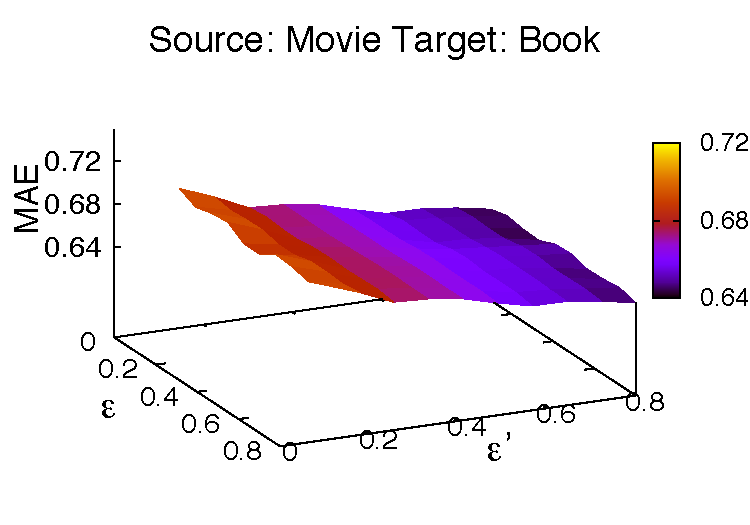
\includegraphics[width=0.23\textwidth,height=0.15\textheight]{figures/Privacy_ib_mb.pdf}}}
\subfigure[\label{fig:privacy_ib_bm}]{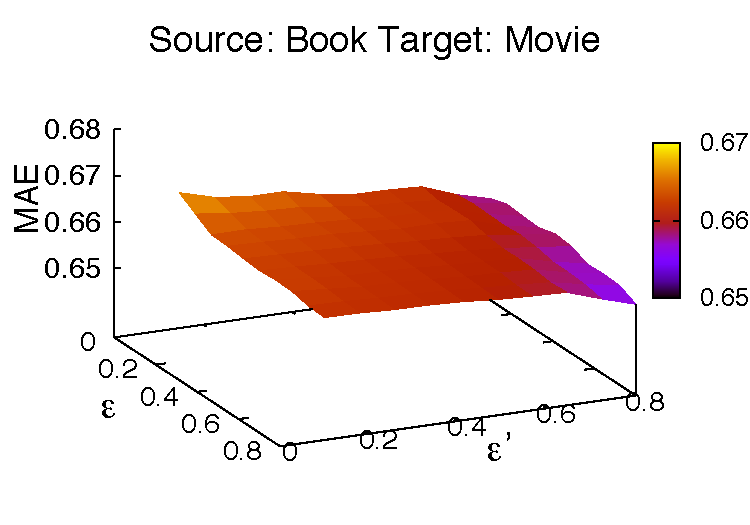
\includegraphics[width=0.24\textwidth,height=0.15\textheight]{figures/Privacy_ib_bm.pdf}}
\vspace{-6mm}
\caption{\bf Privacy trade-off (\crossrecib).}
\vspace{-1mm}
\label{fig:privacy_ib}
\end{figure}


\begin{figure}[ht]
\vspace{-2mm}
\subfigure[\label{fig:privacy_ub_mb}]{\raisebox{0mm}{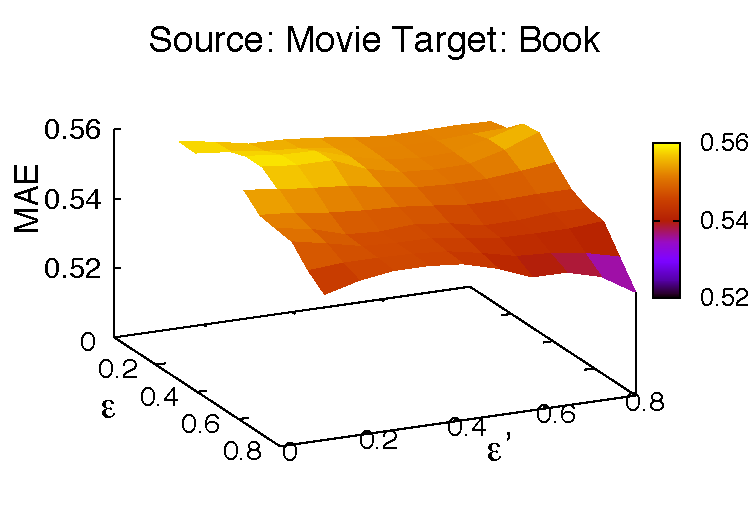
\includegraphics[width=0.23\textwidth,height=0.15\textheight]{figures/Privacy_ub_mb.pdf}}}
\subfigure[\label{fig:privacy_ub_bm}]{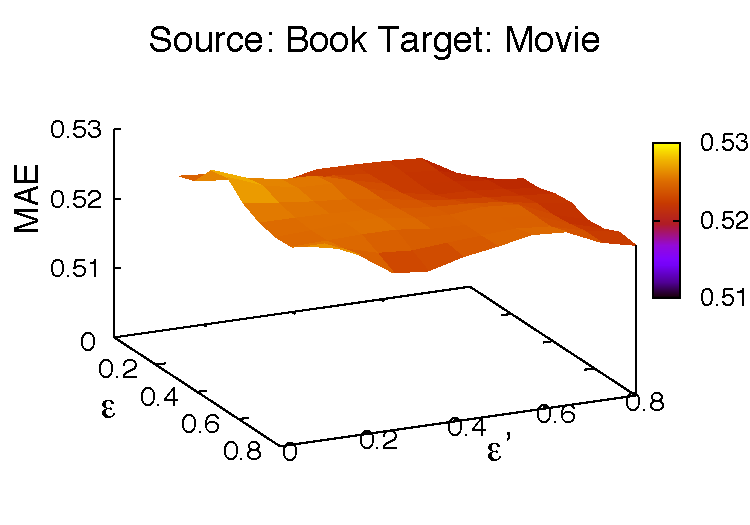
\includegraphics[width=0.24\textwidth,height=0.15\textheight]{figures/Privacy_ub_bm.pdf}}
\vspace{-6mm}
\caption{\bf Privacy trade-off (\crossrecub).}
\label{fig:privacy_ub}
\end{figure}


\subsection{Accuracy}
\label{eval:accuracy}
We now compare the accuracy of the predictions of \crossrec and \npcrossrec with the competitors.

\noindent{\bf Impact of top-k neighbors.}
First, we evaluate the quality in terms of MAE when the size of $k$ (neighbors in Equation~\ref{pred_ib_cf_time}) is varied. Figure~\ref{fig:Book2Movievaryk} demonstrates that \crossrecub and \npcrossrecub outperform the competitors by a significant margin of 30\% where the source domain is book and the target domain is movie. Also, Figure~\ref{fig:Movie2Bookvaryk} shows that \crossrecub and \crossrecib perform slightly better than the non-private competitors whereas \npcrossrec again outperforms the competitors by a margin of 18\% where the source domain is movie and the target domain is book. For all further experiments we consider $k$ as 50.

\begin{figure}[ht]
\vspace{-3mm}
\subfigure[\it \small Source:Book, Target:Movie \label{fig:Book2Movievaryk}]{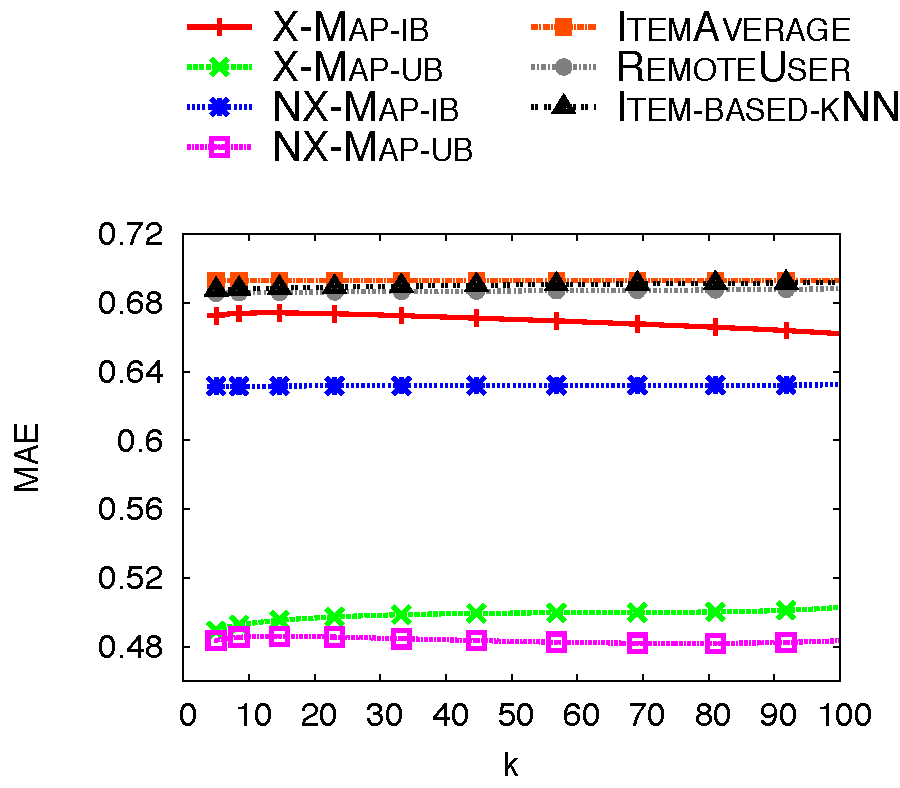
\includegraphics[width=0.245\textwidth,height=0.18\textheight]{figures/MAE_K_original.pdf}}\hspace{-1em}
\subfigure[\it \small Source:Movie, Target:Book \label{fig:Movie2Bookvaryk}]{\raisebox{1.4mm}{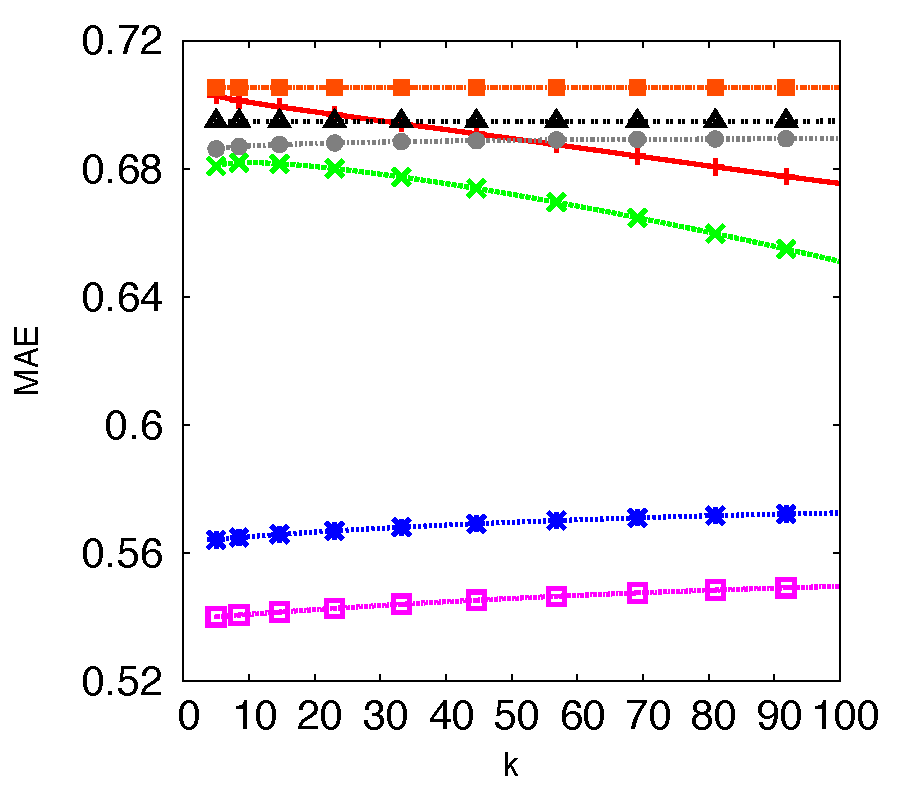
\includegraphics[width=0.245\textwidth,height=0.125\textheight]{figures/MAE_K_swapped.pdf}}}
\vspace{-6mm}
\caption{\bf MAE comparison with varying \emph{k}.}
\vspace{1mm}
\label{fig:varyK}
\end{figure}

\noindent{\bf Impact of overlap.}
Here, we evaluate how \crossrec and \npcrossrec perform when the number of users in the overlap increases. Intuitively, a good approach should provide better accuracy as more and more users connect the domains. These increasing connections improve the baseline heterogeneous similarities which are then leveraged by \graphsim. Figure~\ref{fig:varyTrain} shows that the prediction error of \crossrec decreases as there are more users connecting the domains. Furthermore, we observe in Figure~\ref{fig:Book2MovievaryTrain} that user-based models show more improvement than item-based ones. This behaviour occurs as item similarities are supposed to be more stable than user similarities~\cite{jannach2010recommender}.
%Note that the books domain is more dense than the movies domain, which leads better improvement in prediction quality with an increase in the overlap size as shown in Figure~\ref{fig:Book2MovievaryTrain}.

\begin{figure}[ht]
\vspace{-4mm}
\subfigure[\it \small Source:Book, Target:Movie \label{fig:Book2MovievaryTrain}]{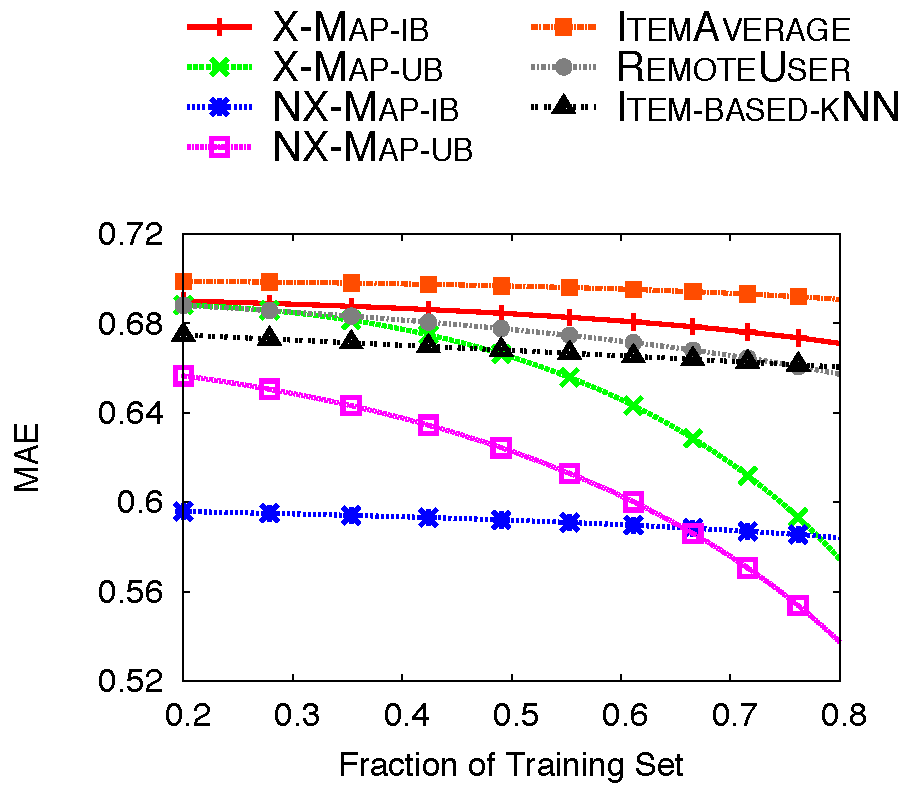
\includegraphics[width=0.245\textwidth,height=0.18\textheight]{figures/MAE_train_original.pdf}}\hspace{-1em}
\subfigure[\it \small Source:Movie, Target:Book \label{fig:Movie2BookvaryTrain}]{\raisebox{1.2mm}{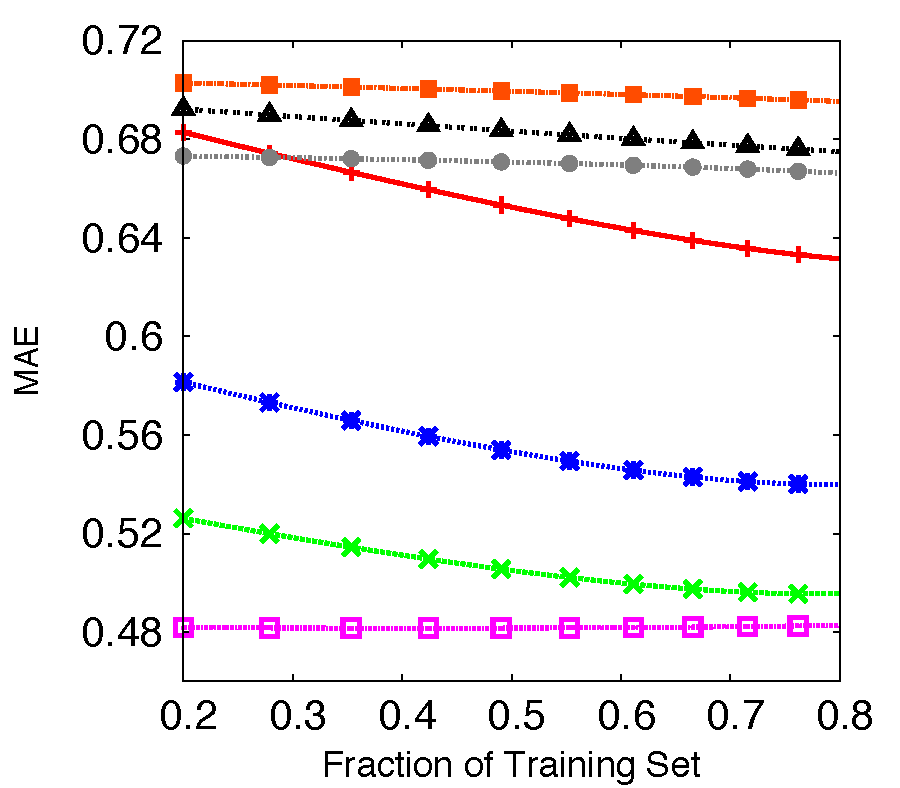
\includegraphics[width=0.245\textwidth,height=0.128\textheight]{figures/MAE_train_swapped.pdf}}}
\vspace{-6mm}
\caption{\bf MAE comparison (Overlap size).\protect\footnotemark}
\label{fig:varyTrain}
\end{figure}

\noindent{\bf Impact of sparsity.}
Next, we evaluate how \crossrec performs when the size of the test profile, in the target domain, increases from a minimum of 0 (cold-start situation) to a maximum of 6 (low sparsity). This experiment also demonstrates the performance of \crossrec when the sparsity of the dataset decreases. Additionally, we evaluate the accuracy improvement of \crossrec over a single domain solution, \emph{item-based kNN in target domain} denoted by \textsc{KNN-sd}, as well over a heterogeneous solution, \emph{item-based kNN in aggregated domain} denoted by \textsc{KNN-cd}. Figure~\ref{fig:varyProfile} demonstrates that \textsc{KNN-sd} and \textsc{KNN-cd} are outperformed by \npcrossrec and \crossrec. Furthermore, we observe a relatively fast improvement for our non-private item-based technique (\npcrossrecib) due to the improvement in item similarities with lower sparsity.
\begin{figure}[ht]
\vspace{-4mm}
\subfigure[\it \small Source:Book, Target:Movie \label{fig:Book2MovievaryProfile}]{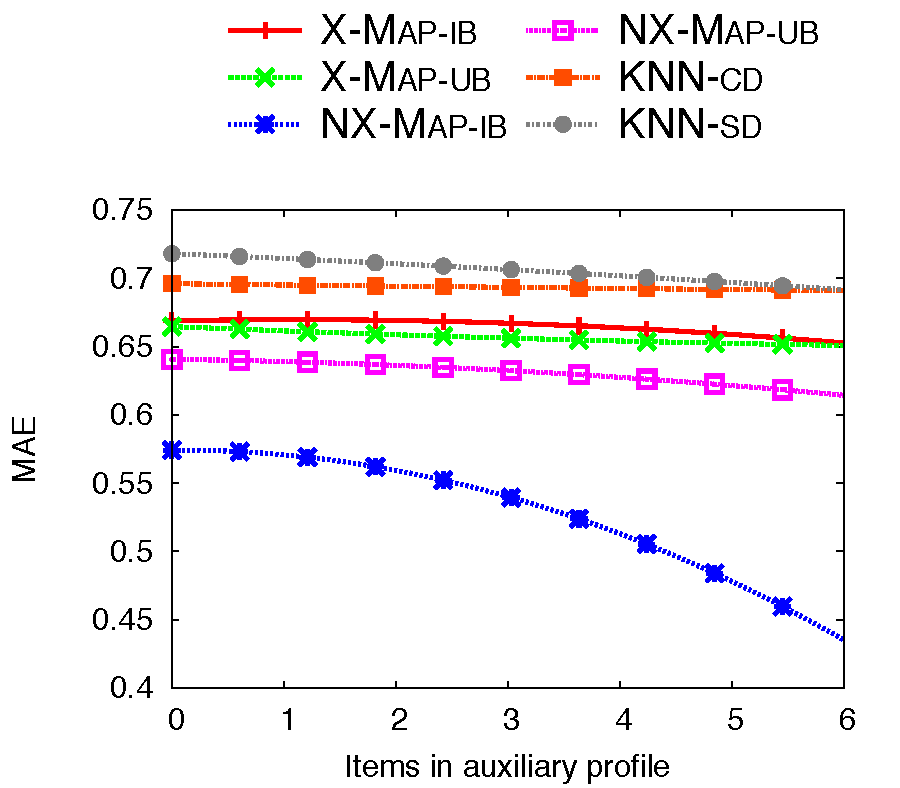
\includegraphics[width=0.245\textwidth,height=0.18\textheight]{figures/MAE_cold_start_original.pdf}}\hspace{-1em}
\subfigure[\it \small Source:Movie, Target:Book \label{fig:Movie2BookvaryProfile}]{\raisebox{1.1mm}{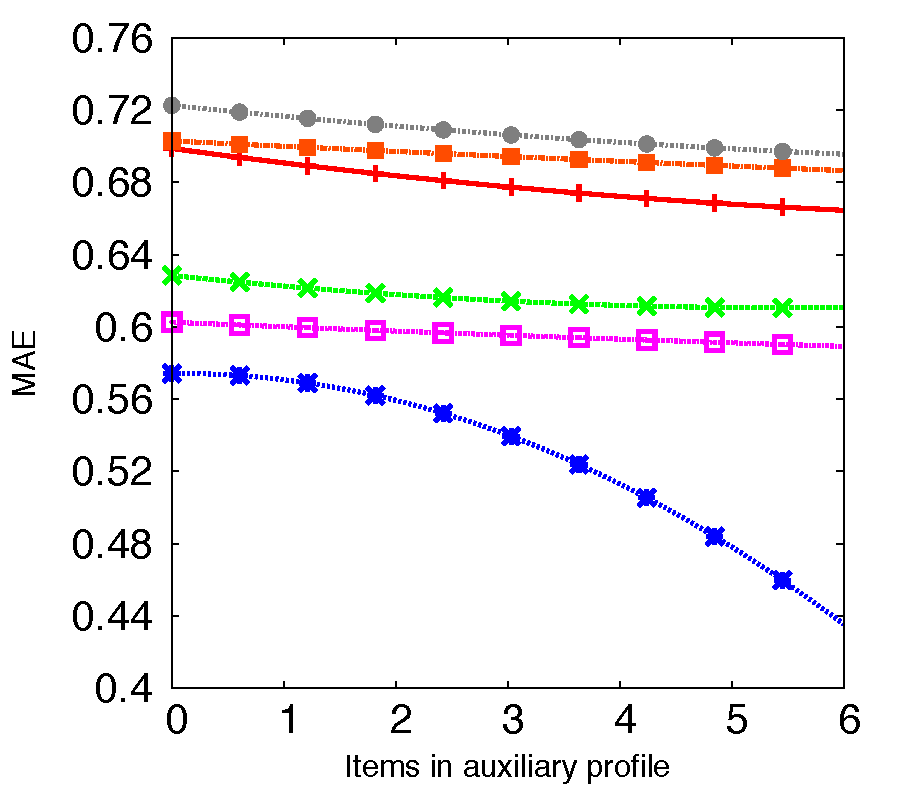
\includegraphics[width=0.245\textwidth,height=0.134\textheight]{figures/MAE_cold_start_swapped.pdf}}}
\vspace{-6mm}
\caption{\bf MAE comparison based on profile size.}
\vspace{2mm}
\label{fig:varyProfile}
\end{figure}

%footnote for overlap size (moved due to page constraint)
\footnotetext{Training set size denotes overlap size.}


\subsection{Scalability}
In this section, we evaluate the scalability of \crossrec in terms of the speedup achieved with an increasing number of computational nodes. We also compare our scalability with a state-of-the-art homogeneous recommender leveraging Spark to implement \emph{Alternating-Least-Squares} based matrix factorization (\textsc{MLlib-ALS}). For the ALS recommender, we use the aggregated ratings over both the domains (Linked-domain personalization). Figure~\ref{fig:scalability} demonstrates the near-linear speedup of \crossrec. Additionally, we see that \crossrec outperforms the scalability achieved by \textsc{MLlib-ALS}.

\begin{figure}[ht]
\vspace{-2mm}
\begin{center}
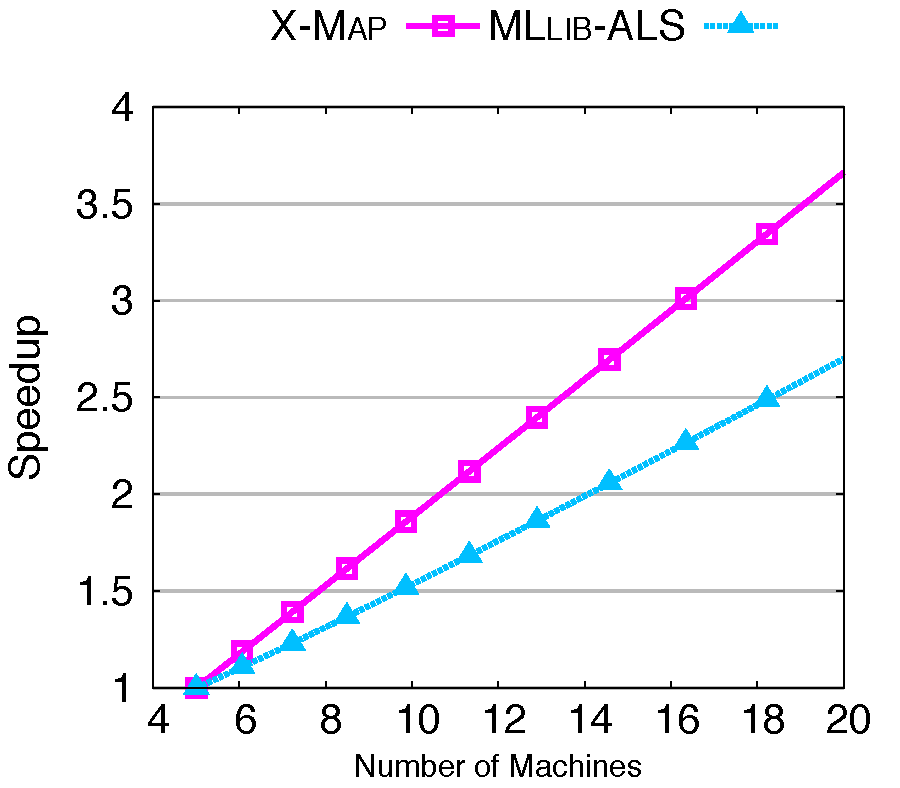
\includegraphics[height=1.3in,width=2in]{figures/Scalability.pdf}
\vspace{-4mm}
\caption{{\bf Scalability of \crossrec.}}
\vspace{-6mm}
\label{fig:scalability}
\end{center}
\end{figure}


\subsection{Online Deployment}
We deployed an online recommendation platform (\url{http://x-map.work/}) leveraging \graphsim and made it available to users. We observe that this recommender is able to recommend books like \emph{Shutter Island: A Novel} when the user queries for the movie \emph{Inception}. Besides, it also recommends the \emph{Shutter Island} movie as a homogeneous recommendation. We observe similar results for multiple other queries. Hence, \graphsim is significantly efficient in achieving heterogeneous personalization in practise.


\iffalse
We deployed a real-time recommender implementing the underlying \graphsim and made it available to internet users. We collected user feedback for a duration of one week which is summarized in Figure~\ref{fig:feedback}. The x-axis denotes the score, provided by the user, in terms of a rating scale ($1$-$5$) with increment of 0.5 and the y-axis denotes the percentage of the total number of users. This preliminary study shows that the user satisfaction level is high.

\begin{figure}[ht]
\vspace{-4mm}
\begin{center}
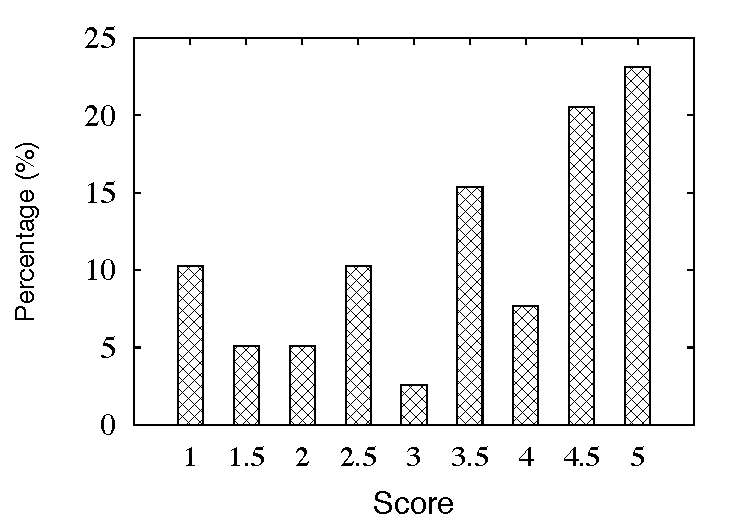
\includegraphics[height=1.3in,width=2in]{figures/Feedback_Frac.pdf}
\vspace{-4mm}
\caption{{\bf Feedback from $51$ users over 1 week.}}
\label{fig:feedback}
\end{center}
\end{figure}
\fi
\vspace{-2mm}
\section{Related Work}
\label{RelWorks}

\noindent{\bf Heterogeneous trends.}
Research on heterogeneous personalization is relatively new. There has been however a few approaches to tackle the problem which we discuss below.
% along with their drawbacks for a real-world deployment. 

%We summarize their characteristics in Table~\ref{fig:relworks}. 
%The main research trends in heterogeneous recommendation were identified by Loizou in his doctoral thesis~\cite{loizou2009recommend} which are as follows.

{\it Smart User Models.} Gonz{\'a}lez et. al introduced the notion of Smart User Models (SUMs)~\cite{gonzalez2005multi}. The idea is to aggregate heterogeneous information to build user profiles that are applicable across different domains. SUMs relies on users' emotional context which are however difficult to capture. Additionally, it has been shown that users' ratings vary frequently with time depending on their emotions~\cite{amatriain2009like}.

{\it Web Monitoring.} 
% Web user agents construct user profiles by monitoring their web activity across different domains. 
Hyung et. al designed a web agent which profiles user interests across multiple domains and leverage this information for personalized web support~\cite{kook2005profiling}. Tuffield et. al proposed Semantic Logger, a meta-data acquisition web agent that collects and stores any information (from emails, URLs, tags) accessed by the users~\cite{tuffield2006semantic}. However, web agents are considered a threat to users' privacy as users' data over different e-commerce applications are stored in a central database administered by the web agent.

{\it Cross-domain Mediation.} Berkovsky et. al~\cite{berkovsky2007cross} proposed the idea of cross-domain mediation to compute recommendations by aggregating data over several recommenders. We showed empirically that \crossrec  outperforms cross-domain mediation in Figures~\ref{fig:varyK} and \ref{fig:varyTrain}.

In contrast, \crossrec introduces a new trend in heterogeneous personalization where the user profile from a source domain is leveraged to generate an \emph{artificial} private or non-private AlterEgo profile in a target domain. The AlterEgo profiles can even be exchanged between e-commerce companies like Netflix, Last.fm due to the privacy guarantee in \crossrec.

\noindent{\bf Merging preferences.} One could also view the 
problem as that of merging single-domain user preferences. Through this angle, several approaches can be considered.

{\it Rating aggregation.} This approach is based on aggregating user ratings over several domains into a single multi-domain rating matrix~\cite{berkovsky2007distributed,winoto2008if, berkovsky2007cross}. Berkovsky et. al showed that this approach can tackle cold-start problems in collaborative filtering~\cite{berkovsky2007distributed}. We showed empirically that \crossrec easily outperforms such rating aggregation based approaches~\cite{berkovsky2007cross}.

{\it Common representation.} This approach is based on a common representation of user preferences from multiple domains either in the form of a \emph{social tag}~\cite{szomszor2008correlating,szomszor2008semantic} or \emph{semantic relationships between domains}~\cite{loizou2009recommend}. Shi et. al developed a Tag-induced  Cross-Domain Collaborative Filtering (TagCDCF) to overcome cold-start problems in collaborative filtering~\cite{shi2011tags}. TagCDCF exploits shared tags to link different domains. They thus need additional tags to bridge the domains. \crossrec can bridge the domains based on the ratings provided by users using its novel \graphsim measure without requiring any such additional information which might be difficult to collect in practice.

{\it Linked preferences.} This approach is based on linking user preferences in several domains~\cite{nakatsuji2010recommendations, cremonesi2011cross}. We showed empirically that \crossrec  outperforms such linked preference based approaches~\cite{cremonesi2011cross} in Figures~\ref{fig:varyK} and \ref{fig:varyTrain}.

{\it Domain-independent features.} This approach is based on mapping user preferences to domain-independent features like \emph{personality features}~\cite{cantador2013relating} or \emph{user-item interaction features}~\cite{loni2014cross}. This approach again requires additional information like \emph{personality scores} which might not be available for all users. 


%\crossrec improves the rating aggregation and linked preferences approaches and uses them along with the \emph{AlterEgo representation} to provide improved heterogeneous recommendations.













\iffalse
\begin{table*}
\begin{center}
\begin{tabular}{ |c|c|c| }
   \hline
 {\bf User Overlap} & {\bf Item overlap} & {\bf User-Item overlap} \\
   \hline
  

{\bf \crossrec} & Stewart et al. 2009~\cite{stewart2009cross} &Berkovsky et al. 2007~\cite{berkovsky2007distributed} \\
  Loni et al. 2014~\cite{loni2014cross} &- & Tiroshi et al. 2012~\cite{tiroshi2012domain} \\


    \hline
\end{tabular}
\end{center}
\vspace{-4mm}
\caption{\bf Related works based on overlap.}
  \label{fig:relworks}
\vspace{-3mm}
\end{table*}
\fi
\vspace{-3mm}
\section{Concluding Remarks}
\label{Conclusion}
We presented \crossrec, a scalable and private heterogeneous recommender. 
\crossrec leverages a novel similarity metric \graphsim, identifying similar items across domains, to generate AlterEgo profiles of users in a domain where they might not have any activity yet. We presented private as well as non-private versions of \crossrec: both perform better in terms of recommendation quality than alternative heterogeneous recommenders~\cite{baltrunas2009context,lemire2005slope,berkovsky2007cross,sarwar2001item, cremonesi2011cross}. (Although, not surprisingly, there is a trade-off between quality and privacy). 

%To conclude, it is important to notice that we addressed the heterogeneous recommendation problem leveraging \emph{user overlap}. The heterogeneous recommendation with \emph{no overlap} between the domains   remains an open problem~\cite{cremonesi2014cross}.












% The following two commands are all you need in the
% initial runs of your .tex file to
% produce the bibliography for the citations in your paper.
\bibliographystyle{abbrv}
{\scriptsize
\bibliography{bib}}  % vldb_sample.bib is the name of the Bibliography in this case
% You must have a proper ".bib" file
%  and remember to run:
% latex bibtex latex latex
% to resolve all references

%\subsection{References}
%Generated by bibtex from your ~.bib file.  Run latex,
%then bibtex, then latex twice (to resolve references).
%\section{Appendix}
\label{appendix}
\subsection{Recommendation-aware sensitivity}
\label{sensitivity}
\begin{definition}[Local Sensitivity]
For a given function $f: \mathcal{R} \rightarrow R$ and a dataset $D$, the Local Sensitivity of $f$ is defined as $LS_f = \max \limits_{D'}\Arrowvert f(D) - f(D')\Arrowvert_1$, where $D$ and $D'$ are neighboring datasets which differ at one user profile. 
\end{definition}

\begin{definition}[Recommendation-aware sensitivity]
Given a score function $q: \mathcal{R} \rightarrow R$ and a dataset $D$, we define the recommendation-aware sensitivity corresponding to a score function $q_i(I,t_j)$ for a pair of items $t_i$ and $t_j$ as:
\begin{flalign*}
&RS(t_i, t_j) = max \{ max_{u_x \in U_{ij}} (\frac{r_{t_{xi}} \times r_{t_{xj}}}{\parallel r'_{t_i} \parallel \times \parallel r'_{t_j} \parallel}),&
\end{flalign*}

\begin{flalign*}
& max_{u_x \in U_{ij}} (\frac{r_{t_i} \cdot r_{t_j}} {\parallel r'_{t_i} \parallel \times \parallel r'_{t_j} \parallel} - \frac{r_{t_i} \cdot r_{t_j}} {\parallel r_{t_i} \parallel \times \parallel r_{t_j} \parallel})\} &
\end{flalign*}
\end{definition}



\begin{proof}
Now, we provide the proof of the recommendation-aware sensitivity. First, we have:
\begin{align*}
RS(t_i, t_j) &= 
max \parallel s(t_i, t_j) - s'(t_i, t_j)\parallel_1
\end{align*}

Next, we insert the similarity values for $s(t_i, t_j)$. A rating vector $r_{t_i} = \lbrack r_{t_{ai}}, ..., r_{t_{xi}}, r_{t_{yi}} \rbrack$ consists of all the ratings for an item $t_i$. Note that here a rating $r_{t_{xi}}$ denotes the result after subtracting the average rating of user $x$ ($\bar{r_x}$) from the actual rating provide by $x$ for an item $i$. Now, we have:
\begin{flalign*}
& s(t_i, t_j) - s'(t_i, t_j) = \frac{r_{t_i} \cdot r_{t_j}}{\parallel r_{t_i} \parallel \times \parallel r_{t_j} \parallel} - 
\frac{r'_{t_i} \cdot r'_{t_j}}{\parallel r'_{t_i} \parallel \times \parallel r'_{t_j} \parallel} &
\end{flalign*}

\begin{flalign*}
& \frac{r_{t_i} \cdot r_{t_j} \times \parallel r'_{t_i} \parallel \times \parallel r'_{t_j} \parallel -
r'_{t_i} \cdot r'_{t_j} \times \parallel r_{t_i} \parallel \times \parallel r_{t_j} \parallel 
}{\parallel r_{t_i} \parallel \times \parallel r_{t_j} \parallel \times \parallel r'_{t_i} \parallel \times \parallel r'_{t_j} \parallel}=\frac{P}{Q} &
\end{flalign*}

Now, we assume that the profile of a user $x$, in $D$, is not present in $D'$. This user rated both $t_i$ and $t_j$. Note that if this user rated one of these items or none, then the similarity value does not depend on the presence or absence of this user in the dataset. Hence, we have: $\parallel r'_{t_i} \parallel \times \parallel r'_{t_j} \parallel \leq \parallel r_{t_i} \parallel \times \parallel r_{t_j} \parallel$. 

Now, we have P= ($r_{t_i} \cdot r_{t_j} \times \parallel r'_{t_i} \parallel \times \parallel r'_{t_j} \parallel -
r'_{t_i} \cdot r'_{t_j} \times \parallel r_{t_i} \parallel \times \parallel r_{t_j} \parallel$) and Q=($\parallel r_{t_i} \parallel \times \parallel r_{t_j} \parallel \times \parallel r'_{t_i} \parallel \times \parallel r'_{t_j} \parallel$).
Hence, $Q \geq 0$ and depending on whether $P \geq 0$ or $P \leq 0$ we have two conditions which are as follows.

If $P \geq 0$, then we have:
\begin{flalign*}
&\parallel s(t_i, t_j) - s'(t_i, t_j) \parallel_1&
\end{flalign*}

\begin{flalign*}
&=\frac{r_{t_i} \cdot r_{t_j} \times \parallel r'_{t_i} \parallel \times \parallel r'_{t_j} \parallel -
r'_{t_i} \cdot r'_{t_j} \times \parallel r_{t_i} \parallel \times \parallel r_{t_j} \parallel 
}{\parallel r_{t_i} \parallel \times \parallel r_{t_j} \parallel \times \parallel r'_{t_i} \parallel \times \parallel r'_{t_j} \parallel} &
\end{flalign*}

\begin{flalign*}
& \leq \frac{(r_{t_i} \cdot r_{t_j} - r'_{t_i} \cdot r'_{t_j}) \times \parallel r_{t_i} \parallel \times \parallel r_{t_j} \parallel}
{\parallel r_{t_i} \parallel \times \parallel r_{t_j} \parallel \times \parallel r'_{t_i} \parallel \times \parallel r'_{t_j} \parallel} &
\end{flalign*}

\begin{flalign*}
&= \frac{(r_{t_i} \cdot r_{t_j} - r'_{t_i} \cdot r'_{t_j})}
{\parallel r'_{t_i} \parallel \times \parallel r'_{t_j} \parallel}&
\end{flalign*}

If $P \leq 0$, then we have:
\begin{flalign*}
& \parallel s(t_i, t_j) - s'(t_i, t_j) \parallel_1 &
\end{flalign*}

\begin{flalign*}
&=
\frac{r'_{t_i} \cdot r'_{t_j} \times \parallel r_{t_i} \parallel \times \parallel r_{t_j} \parallel - r_{t_i} \cdot r_{t_j} \times \parallel r'_{t_i} \parallel \times \parallel r'_{t_j} \parallel }
{\parallel r_{t_i} \parallel \times \parallel r_{t_j} \parallel \times \parallel r'_{t_i} \parallel \times \parallel r'_{t_j} \parallel} &
\end{flalign*}

\begin{flalign*}
& = \frac{(r_{t_i} \cdot r_{t_j} - r_{t_{xi}} \times r_{t_{xj}}) \times \parallel r_{t_i} \parallel \times \parallel r_{t_j} \parallel - r_{t_i} \cdot r_{t_j} \times \parallel r'_{t_i} \parallel \times \parallel r'_{t_j} \parallel}
{\parallel r_{t_i} \parallel \times \parallel r_{t_j} \parallel \times \parallel r'_{t_i} \parallel \times \parallel r'_{t_j} \parallel} &
\end{flalign*}

\begin{flalign*}
&= \frac{r_{t_i} \cdot r_{t_j} \times (\parallel r_{t_i} \parallel \times \parallel r_{t_j} \parallel  - \parallel r'_{t_i} \parallel \times \parallel r'_{t_j} \parallel)}
{\parallel r_{t_i} \parallel \times \parallel r_{t_j} \parallel \times \parallel r'_{t_i} \parallel \times \parallel r'_{t_j} \parallel}  &
\end{flalign*}


\begin{align*}
& - \frac{r_{t_{xi}} \times r_{t_{xj}} \times \parallel r_{t_i} \parallel \times \parallel r_{t_j} \parallel}{\parallel r_{t_i} \parallel \times \parallel r_{t_j} \parallel \times \parallel r'_{t_i} \parallel \times \parallel r'_{t_j} \parallel}&
\end{align*}

\begin{flalign*}
& \leq \frac{r_{t_i} \cdot r_{t_j} \times (\parallel r_{t_i} \parallel \times \parallel r_{t_j} \parallel  - \parallel r'_{t_i} \parallel \times \parallel r'_{t_j} \parallel)}
{\parallel r_{t_i} \parallel \times \parallel r_{t_j} \parallel \times \parallel r'_{t_i} \parallel \times \parallel r'_{t_j} \parallel}&
\end{flalign*}

\begin{flalign*}
&=\frac{r_{t_i} \cdot r_{t_j}} {\parallel r'_{t_i} \parallel \times \parallel r'_{t_j} \parallel} - \frac{r_{t_i} \cdot r_{t_j}} {\parallel r_{t_i} \parallel \times \parallel r_{t_j} \parallel}&
\end{flalign*}

Hence, we have the recommendation-aware sensitivity as:
\begin{flalign*}
&RS(t_i, t_j) = max \{ max_{u_x \in U_{ij}} (\frac{r_{t_{xi}} \times r_{t_{xj}}}{\parallel r'_{t_i} \parallel \times \parallel r'_{t_j} \parallel}),&
\end{flalign*}

\begin{flalign*}
& max_{u_x \in U_{ij}} (\frac{r_{t_i} \cdot r_{t_j}} {\parallel r'_{t_i} \parallel \times \parallel r'_{t_j} \parallel} - \frac{r_{t_i} \cdot r_{t_j}} {\parallel r_{t_i} \parallel \times \parallel r_{t_j} \parallel})\} &
\end{flalign*}
\end{proof}




\end{document}
